\documentclass{article}

\usepackage{PRIMEarxiv}

\usepackage[utf8]{inputenc} % allow utf-8 input
\usepackage[T1]{fontenc}    % use 8-bit T1 fonts
\usepackage{hyperref}       % hyperlinks
\usepackage{url}            % simple URL typesetting
\usepackage{booktabs}       % professional-quality tables
\usepackage{amsfonts}       % blackboard math symbols
\usepackage{nicefrac}       % compact symbols for 1/2, etc.
\usepackage{microtype}      % microtypography
\usepackage{fancyhdr}       % header
\usepackage{graphicx}       % graphics
\usepackage{longtable}      % paginate long tables
%\usepackage{natbib}
\usepackage[numbers]{natbib}
\usepackage{amsmath}
\usepackage{wrapfig}
\usepackage{doi}
%\usepackage{moreverb}
% add a little more space between hlines in the tables
%\usepackage{tabularx}
%\setlength{\extrarowheight}{1pt}

%Header
\pagestyle{fancy}
\thispagestyle{empty}
\rhead{ \textit{ }} 

% Update your Headers here
\fancyhead[LO]{Evaluating ASR Hallucinations}
% \fancyhead[RE]{Firstauthor and Secondauthor} % Firstauthor et al. if more than 2 - must use \documentclass[twoside]{article}

%\newcommand\BibTeX{{\rmfamily B\kern-.05em %\textsc{i\kern-.025em b}\kern-.08em
%T\kern-.1667em\lower.7ex\hbox{E}\kern-.125emX}}


\title{Evaluating Hallucination Characteristics of Automated Speech Recognition Systems
%%%% Cite as
%%%% Update your official citation here when published 
\thanks{\textit{\underline{Citation}}: 
\textbf{Authors. Title. Pages.... DOI:000000/11111.}} 
}

\author{ 
    \href{https://orcid.org/0000-0002-1254-5943}{
\includegraphics[scale=0.06]{orcid.pdf}
    \hspace{1mm}Robert F. Dougherty, PhD}\\
	Soundtrip Health\\
	  Portland, OR, USA \\
	\texttt{bob@soundtrip.health} \\
	\And
	\href{https://orcid.org/0009-0004-4740-9126}{
\includegraphics[scale=0.06]{orcid.pdf}
    \hspace{1mm}Mario Shafiei, MSc} \\
	  Reno, NV, USA \\
	\texttt{mario.shafiei@gmail.com}
	\And
	\href{https://orcid.org/0000-0000-0000-0000}{
\includegraphics[scale=0.06]{orcid.pdf}
    \hspace{1mm}Merve Alti, MSc} \\
	  London, UK \\
	\texttt{merveatli@outlook.com}
	\And
	\href{https://orcid.org/0009-0003-8387-8475}{
\includegraphics[scale=0.06]{orcid.pdf}
    \hspace{1mm}Carly Leininger} \\
	  Mill Valley, CA, USA \\
	\texttt{carly.leininger@gmail.com}
	\And
	\href{https://orcid.org/0000-0001-6215-7343}{
\includegraphics[scale=0.06]{orcid.pdf}
    \hspace{1mm}Patrick Staples, PhD} \\
	  Oakland, CA, USA \\
	\texttt{ctphoenix@gmail.com}
}

%%% Add PDF metadata. You can check the metadata with 'pdfinfo thisfile.pdf'
\hypersetup{
pdftitle={Hallucination Characteristics of Automated Speech Recognition Systems},
pdfsubject={q-bio.NC, q-bio.QM},
pdfauthor={Robert F.~Dougherty},
pdfkeywords={Automated Speech Recognition, Healthcare, ASR Hallucination, Signal-to-noise, ASR benchmark},
}

\begin{document}
\maketitle

\begin{abstract}
Advances in machine learning offer opportunities for transforming the healthcare industry. While automated speech recognition (ASR) systems are becoming ubiquitous and their transcription accuracy equals or exceeds human performance under ideal conditions, these systems can produce significant errors in noisy acoustic environments. Despite extensive research on ASR performance, there remains a critical gap in understanding how modern generative models respond to varied background noise, especially music. This paper presents a systematic analysis of ASR error patterns across multiple state-of-the-art systems, including recent open-source models and commercial offerings. Using the AMI meeting corpus as our primary test data, we manipulated signal-to-noise ratios (SNR) across a 40dB range with two different types of background noise: office noise and instrumental music. By comparing ASR outputs against human-verified transcripts, we identified distinct patterns of errors that emerge as acoustic conditions degrade. Our results reveal that while the four ASR systems tested perform well on standard word-error metrics, they exhibit markedly different failure modes, with some more prone to producing fluent but fabricated content (hallucinations), particularly when transcribing audio containing background music. We examine these errors in detail using a novel time-constrained transcript alignment algorithm and quantify the prevalence of the various error types across different acoustic conditions. These findings have substantial implications for real-world applications, particularly in environments where background noise and music are common, such as in mental health treatment sessions. Our work provides valuable insights for both ASR system developers seeking to improve robustness and end-users needing to understand system limitations in various acoustic conditions. We also make available an open-source ASR evaluation framework that can be used to continue to evaluate new ASR systems to determine which have failure modes that are the best fit for a given application.

%Recent advances in automated speech recognition (ASR) systems have dramatically improved transcription accuracy under ideal conditions. However, these systems can produce significant errors and hallucinations (i.e., generating text that is not supported by the audio data). We have found that the probability of models producing hallucinations is increased when processing speech in challenging acoustic environments, especially those that include background music. This paper presents a systematic analysis of ASR error patterns across multiple state-of-the-art systems, including both recent open-source models and commercial systems currently on the market. The primary focus is on their behavior under varying levels of background noise, where such "noise" includes any non-speech sound, including background music. Using the AMI meeting corpus as our primary test data, we manipulated signal-to-noise ratios (SNR) across a 40dB range with two different types of background noise; office noise and instrumental music. By comparing ASR outputs against human-verified transcripts, we identified distinct patterns of errors, including hallucinations, that emerge as acoustic conditions degrade, particularly in the context of background music. Our results reveal that while modern generative ASR systems outperform previous generations of ASR systems on overall error metrics, they exhibit markedly different failure modes, often producing fluent text for portions of audio that contain no intelligible speech [Will we not mention any numbers related to WER?]. These hallucination errors are particularly problematic for common use cases, such as transcription of dialog recorded in noisy office settings. We present a taxonomy of hallucination error types and discuss their implications for real-world applications, particularly in environments where background noise and overlapping speech are common. These settings include mental health uses such as transcribing any dialog that occurs during psychedelic treatment sessions, where background music is often playing. These findings provide valuable insights for both ASR system developers and end-users in understanding system limitations and reliability under various acoustic conditions. 
\end{abstract}


% keywords can be removed
\keywords{Automated Speech Recognition 
\and Healthcare
\and ASR Hallucination 
\and Signal-to-noise
\and ASR benchmark}


\section{Introduction}

Automated speech recognition (ASR) systems are increasingly deployed in mental health care to convert patient-therapist dialogues into analyzable text, enabling the automation of therapist evaluation and fidelity monitoring of the care provided, as well as providing features for predictive modeling of therapeutic outcomes. For example, machine learning (ML) models using natural language processing (NLP) features extracted from patient dialog have demonstrated utility in predicting symptom trajectories and treatment response \cite{dougherty2023psilocybin,cohen2024evaluating,siegel2024enrichment}. However, the real-world word error rate (WER) for ASRs used to transcribe psychotherapy audio acquired in typical clinical settings has been reported to be 25\% \cite{miner2020asrpsychotherapy}. Such a high error rate will impede the incorporation of NLP features into a precision psychiatry platform until critical gaps in accuracy, environmental noise resilience, and clinical context awareness are measured and improved. The ASR accuracy challenges are even more acute for mental health dialog that takes place with music playing in the background, as is the case for music therapy, some ketamine treatments, and some psychedelic-assisted therapies that are currently undergoing clinical trials.\cite{kaelen2018hidden,carhart2018psychedelics,jerotic2024psychedelia}. Background music, a potentially therapeutic tool in these types of treatments, may degrade transcription quality \cite{malek2017musicasr,malek2018musicasr} and thus propagate errors into downstream predictive models.

This analysis will provide both quantitative and qualitative insights into the accuracy of ASR-generated transcript word and timestamp errors by comparing transcripts generated by several state-of-the-art ASR models with ground-truth human transcripts. While we would prefer to run this analysis on real-world mental health recordings, such data are sensitive and thus there are no useful open-source data. Therefore, we selected an open source ASR dataset and simulate real-world clinical conditions. Also, while diarization (labeling who said each word) is crucial for many NLP applications, this analysis will focus on transcription and leave diarization error characteristics for future work. Further, by using open-source data and releasing our corresponding analysis code as open-source software we create an ASR testing framework that can be used to continue to evaluate new ASR systems to determine which might be best fit for a given application given their differing failure modes.

\subsection{Background}

\subsubsection{ASR in Precision Psychiatry}

ASR systems are routinely employed to automate the transcription of psychotherapy sessions, reducing the administrative burden on clinicians while creating searchable records for quality assurance \cite{flemotomos2022asrpsychotherapyquality}. In cognitive-behavioral therapy (CBT) and dialectical behavior therapy (DBT), these transcriptions enable supervisors to evaluate therapists' adherence to standardized interventions-- a critical factor in maintaining treatment fidelity across large-scale implementations \cite{chen2022asrcbtquality}. Commercial cloud-based ASR services currently achieve median WERs of 25\% in psychotherapy contexts, with comparable performance between patient and clinician speech \cite{miner2020asrpsychotherapy}. These high error rates limit the utility of transcripts for important clinical decision making, such as informing safety monitoring or making diagnostic decisions.

The integration of ASR with NLP pipelines has enabled novel applications in predictive analytics for mental health care. By processing session transcripts through sentiment analysis, topic modeling, syntactic pattern recognition, and speech timings, researchers can quantify therapeutic alliance strength \cite{{goldberg2020machine}}, predict depressive symptom trajectories \cite{cohen2024evaluating,li2023sinlp,graham2019aimentalhealth}, and identify markers to predict treatment response \cite{dougherty2023psilocybin,siegel2024enrichment}. Crucially, the clinical utility of these models depends on ASR systems' ability to accurately capture not just lexical content, but paralinguistic elements like speech rhythm and pause duration. Thus, in addition to accurate transcriptions that capture the semantic intent of what is said, capturing accurate word-level timestamps is important for predictive features based on vocal latency\cite{cohen2024evaluating,siegel2024enrichment}.

\subsubsection{Hallucinations}
The term "hallucination" has become common when describing the errors made by generative artificial intelligence (genAI) systems, including ASR systems. However, we argue that not all ASR errors are equivalent and that it is useful to distinguish between isolated single-word errors and the multi-word insertion errors that genAI-based ASRs can produce. These errors are particularly problematic because they add linguistically coherent and context-relevant phrases and sentences that have no basis in the underlying acoustic data. While an isolated single word error may change the meaning of a phrase that is present in the transcript (e.g., omitting a "not"), a genAI "hallucination" can add completely new phrases and sentences to the transcript. For example, Koenecke et al. \cite{Koenecke_2024} evaluated Whisper AI’s speech-to-text transcription API and found hallucinations in 1.4\% of the 187 transcripts. These were not ‘undesirable generated text’ or ‘word errors’ but were complete, linguistically coherent sentences inserted into transcriptions when there was no intelligible speech in the audio files. Thematic analysis showed that nearly 40\% of these hallucinations were harmful in some way, with 19\% including harms perpetuating violence (i.e., physical violence or death, sexual innuendo, or demographic stereotyping), 13\% including harms of inaccurate associations (i.e., made up names, relationships or health statuses), and 8\% including harms of false authority (i.e., fake video evidence and website links) \cite{Koenecke_2024}. These results raise concerns that are particularly acute when these transcriptions will be used in important decision-making. Thus, we define an ASR hallucination as consecutive sequence of three or more word errors whose linguistic coherence is indistinguishable from correctly transcribed content.
%A single word deletion error may be harmless (e.g., omitting a dis-fluency such as "uhm") or may change the entire meaning of a phrase (e.g., omitting a "not").  
%Early ASR researchers sometimes called mistranslations which were semantically and grammatically incorrect as ‘hallucinations’ \cite{lee2019hallucinations}. However, the word hallucination was used much earlier within this field to refer to ‘errors’ \cite{Anguita2005,Sagae2012} or the word ‘hallucinated content’ was used \cite{koehn-knowles-2017-six}. Recently, the word ‘hallucination’ has been used and defined in the literature more frequently. Researchers started using the term ‘hallucination’ in the context of Natural Language Generation (NLG) to refer to ‘unfaithful’ or ‘nonsensical’ generations. They differentiated between intrinsic hallucinations (by manipulating the information present in the input document) and extrinsic hallucinations (by adding information not directly inferable from the input document) \cite{maynez2020faithfulnessfactualityabstractivesummarization}. This term also became widely adapted within the context of LLMs, some researchers adopted the former definition \cite{kaddour2023challengesapplicationslargelanguage}, some defined it as ‘the phenomenon in which LLMs provide information, which is incorrect or inappropriate, presented as a fact’ \cite{mckenna-etal-2023-sources} or as ‘produced outputs that are seemingly plausible but deviate from factual knowledge sources’ \cite{zhang2023sirenssongaiocean}. It has also been adapted within the STTs context, as 'undesirable text that is nonsensical, or unfaithful to the provided source input' \cite{Koenecke_2024}, or as ‘fluent and coherent outputs of neural models entirely disconnected from the input’ \cite{frieske2024hallucinations}.  

%Despite the varying definition of hallucination within the literature, there seems to be common ground in which the text generated is incorrect. One could argue that this may not be the correct word to use when referring to errors. The word ‘hallucination’, originates from the Latin word alucinatus, which means "to wander in mind" \cite{???}. A hallucination is a perception in the absence of an external stimulus that has the compelling sense of reality \cite{elmallakh2010hallucinations}. In other words, the experience of something that isn’t there. Interestingly, Koenecke et al. \cite{Koenecke_2024}, evaluated Whisper AI’s speech-to-text transcription API and found hallucinations in 1.4\% of the 187 transcripts. These were not ‘undesirable generated text’ or ‘word errors’ but were complete, linguistically coherent sentences inserted into transcriptions when there was no intelligible speech in the audio files. Thematic analysis showed that nearly 40\% of these hallucinations were harmful in some way, with 19\% including harms perpetuating violence (i.e., physical violence or death, sexual innuendo, or demographic stereotyping), 13\% including harms of inaccurate associations (i.e., made up names, relationships or health statuses), and 8\% including harms of false authority (i.e., fake video evidence and website links) \cite{Koenecke_2024}. These results raise concerns that are particularly acute when these transcriptions will be used in important decision-making. 

%These hallucination errors can stem from common patterns in training data training, overconfidence in model predictions, and unreliable training data \cite{barański2025whisperasrhallucinations}. 
In this paper we examine whether adding background music or noise to audio recordings increases the frequency of transcription errors generally, and hallucinations specifically. We hypothesize that an increase in background music/noise levels will result in more hallucinations and errors, as it becomes more difficult for the ASR model to accurately recognize speech. While previous studies have explored error stimulation through artificial noise injection \cite{frieske2024hallucinations, barański2025whisperasrhallucinations}, our approach differs by using 'natural' noise, such as office sounds and background music, to assess its impact on ASR performance. Unlike Frieske \& Shi \cite{frieske2024hallucinations}, who introduced label mismatches and synthetic perturbations, and Barański et al. \cite{barański2025whisperasrhallucinations}, who examined hallucinations from non-speech audio, our study focuses on how real-world background noise affects ASR hallucinations in practical environments. 

\section{Methods}
Given the focus on mental health ASR applications, analysis of recordings of real therapist-patient dialog would be ideal. However, there is little such open-source data available so we chose to use a corpus of high-quality dialog audio recordings with corresponding human ground-truth transcriptions (the AMI Meeting Corpus \cite{ami2006}) and simulate different different acoustic noise environments by mixing these recordings with two different types of background noise (office noise and instrumental music) across a 40 deci-Bel (dB) signal-to-noise ratio (SNR) range. These audio files were then transcribed using four different state-of-the-art ASR systems with each resulting transcript compared to the ground-truth human verified transcript. We chose the AMI corpus because the dialog includes both spontaneous and semi-scripted dialog among small groups of people, similar to mental health dialog. Also, the audio recordings include speaker-mounted microphones (headset and/or lapel) and thus have very low levels of background noise and acoustic reverberations, forming an ideal auditory base upon which to add background music and noise.

\subsection{Data}
The AMI Meeting Corpus \cite{ami2006} consists of about 100 hours of meeting recordings made with a range of signals synchronized to a common timeline. These include close-talking and far-field microphones, individual and room-view video cameras, and output from a slide projector and an electronic whiteboard. The meetings were conducted in English, but with many non-native speakers, and in three different rooms with different acoustic properties. For this work, we used the recordings made using an audio mix of all the speaker-mounted lapel microphones (labeled "Mix-Lapel" in the AMI audio files) when available, or a mix of the headset microphones (labeled "Mix-Headset" in the audio files) for sessions where the lapel recordings were not available. These two recordings are quite similar and both provide high quality audio of all speakers, with the lapel recordings having a slight benefit due to fewer voice pop events and associated signal clipping. The Corpus also includes high quality, manually produced orthographic transcription for each speaker, including word-level timings derived using an ASR in forced alignment mode \cite{ami2006,rousso2024forcedalignment}.

\subsection{Simulating noisy clinical environments}
To simulate the real world use-cases that are of the most interest to us, we manipulated the AMI audio recordings to add two different types of background noise: instrumental music and unstructured background noise that is likely to be found in a clinical office setting where patient-therapist dialog may be recorded. Both noise types were recorded with an external Jabra USB microphone (model PH50002W) in the same office room. The space is approximately four square meters with hard surfaces and typical office furniture. The dominant noise sources in the space are the hum of air circulation machinery, occasional muffled footsteps from the hallway outside the room, and some street noise from the outdoor urban environment. This acoustic environment was chosen to simulate a private room in a busy medical clinic. The room noise was recorded twice, once with no additional sound added ("office noise") and once with a small speaker (Klipsch The One Plus tabletop speaker) playing instrumental background music at a comfortable listening volume. The music tracks were chosen to be representative of a psychedelic treatment playlist. Both of these noise recordings and the software code used to generate the different SNR simulations, run the ASR transcriptions, and analyze the transcripts are provided in the accompanying source code repository \cite{asr_hallucination}.

The audio mixing was implemented in Python and used PyDub \cite{pydub2018} and Numpy \cite{numpyharris2020} to implement the following algorithm. First, the energy of both the signal and noise were computed as the mean squared value of their respective sample amplitudes:
   \[
   E_{\text{signal}} = \frac{1}{N} \sum_{i=1}^{N} \text{signal}[i]^2
   \]
   \[
   E_{\text{noise}} = \frac{1}{N} \sum_{i=1}^{N} \text{noise}[i]^2
   \]
   where \( N \) is the number of samples.

The gain \( g \) used to adjust the noise level to achieve the target SNR was then calculated based on the desired SNR using the formula:
   \[
   g = \sqrt{10^{-\frac{\text{SNR}}{10}} \cdot \frac{E_{\text{signal}}}{E_{\text{noise}}}}
   \]

Assuming that the signal and noise are uncorrelated, which is guaranteed to be true for our application, we compute the coefficients \( a \) and \( b \) such that the energy of the scaled signal plus the scaled noise matches the energy of the input signal with the following:
   \[
   a = \sqrt{\frac{1}{1 + g^2}}
   \]
   \[
   b = \sqrt{\frac{g^2}{1 + g^2}}
   \]

Finally, the mixed signal was obtained by combining the scaled signal and noise:
   \[
   \text{mixed signal} = a \cdot \text{signal} + b \cdot \text{noise}
   \]


\subsection{ASR Systems}
We selected four ASR systems for this analysis. Two open-source models that we ran locally (WhisperX\cite{whisperxbain2023} and Reverb\cite{reverbbhandari2024}) and two commercial services via their respective APIs (AWS Transcribe\cite{awstranscribe2024} and Assembly AI\cite{assemblyaiuniversal2024}). All transcriptions were run between November 2024 and February 2025 with the latest version of each ASR available at that time. Details of the ASR transcription parameters can be found in the corresponding software code release. The analysis (including the two locally-run open-source models) was performed on a workstation running Ubuntu 24.04LTS Linux on a 6 core AMD Ryzen 5 5600X CPU with 32GB RAM and an NVidia GeForce RTX 5090 GPU. However, the code should run on any modern hardware that supports the python requirements specified in our Github repository \cite{repo}.

\subsection{Quantitative error evaluation}
The following describes the procedure for analyzing the transcription accuracy using the human transcripts as a reference. For more details about ASR accuracy analysis and some recent benchmarks, see \cite{Kuhn_2023}.  

\subsubsection{Transcript Normalization}
The process of normalizing transcripts for error analysis standardizes transcripts to make them more comparable when estimating errors and computing metrics such as word error rate (WER). These normalization steps aim to eliminate superficial differences that don't affect the core content, allowing for a more accurate comparison of transcriptions and evaluation of transcription errors. The normalization steps that we applied follow industry best practices (\cite{radford2022robust}). Specifically, we used whisper-normalizer, an open-source implementation to perform the following three main steps (for details see Appendix C of \cite{radford2022robust}): 

\begin{itemize}
  \item Convert all characters in the transcript to lowercase. Capitalization is generally not relevant to the semantic content. 

  \item Remove any phrases between matching brackets ([, ]) or ((, )). These are generally annotations by the transcriber, such as [laughing]. While many ASR models also add such tags, the likelihood that they will exactly match the tags a human transcriber chooses to use is low (“[laughing]”, “[laughter]”, “[laugh]”, etc.), so the lack of a perfect match should not count as an error. 

  \item Remove any of the following disfluency utterances: hmm, mm, mhm, mmm, uh, um, erm, err, er, m, ah, la, da, ooh, aum, rawr, om. Exactly how a transcriber (human or machine) chooses to code non-words may vary (e.g., um vs. erm) and thus should not count as an error. 
\end{itemize}

\subsubsection{Alignment}
Transcript alignment is the process of matching the words in an ASR transcript to a reference (ground truth) transcript when calculating accuracy metrics such as WER. This alignment ensures that corresponding words in both transcripts are correctly paired for comparison, helping to accurately identify insertions, deletions, and substitutions. This step is crucial because if there are any insertion or deletion errors the two transcripts under comparison will not have corresponding lists of words.  

As an example, if the reference is "I really like apples" and the ASR output is "I love red apples", alignment would pair "I" with "I", "like" with "love" (and tag it as a substitution), and "apples" with "apples" (a match). It would tag “really” as a deletion as the ASR did not include it, and tag “red” as an insertion by the ASR. Alignment makes it possible to count errors systematically. 

\textbf{Word alignment}

Word-based alignment was performed using a variant of the Levenshtein edit distance algorithm (see \cite{brill2001automatically,jiweri2024}), which minimizes the number of operations (insertions, deletions, and substitutions) needed to transform one sequence of words into another. This approach is widely used in ASR evaluation (as well as numerous other fields such as genetics) and detailed in various research papers on speech recognition performance evaluation \cite{brill2001automatically}. 

While word-based alignment algorithms are commonly used to evaluate ASR systems, these algorithms can fail to accurately align the transcripts, especially in the case of audio with low SNR levels and thus high transcription error rates. This occurs because common words that are distant in time might be spuriously aligned. In Section \ref{sec:alignaccuracy} we show examples of such word-alignment errors and evaluate how they impacted error rate metrics. We also describe a simple time-constrained alignment algorithm that addresses these issues.

\textbf{Time-constrained alignment}

To address these limitations of traditional word-based alignment, we implemented a simple time-constrained alignment algorithm that produces more accurate alignments and thus more accurate error metrics. This algorithm selects a candidate set of words in the hypothesis transcript for each word in the reference transcript using a symmetric temporal window around the reference word start and end timestamps to find a potential matching word. If a match is found, the matching word and all temporally prior hypothesis words in the candidate set are removed from any future consideration. Unmatched words and words following a match are returned to the hypothesis sequence to be used for aligning to the next reference words. An implementation of this algorithm is included in the corresponding code release \cite{coderepo}). We should note, however, that while this simple time-constrained algorithm is useful for characterizing error types and quantifying hallucination errors, it does not necessarily produce a globally-optimal alignment that takes into account both temporal distances and word errors and thus future work is needed to develop such an algorithm.  

\subsubsection{Accuracy Metric}
Word Error Rate (WER) is a common metric used to evaluate the accuracy of ASR systems. It measures the difference between an ASR transcript and a reference (ground-truth) transcript by calculating the proportion of word errors (substitutions, deletions, and insertions) relative to the total number of words in the reference transcript. WER is used because it provides a simple, objective measure of transcription performance, making it easy to compare different ASR models based on how accurately they transcribe speech. The WER formula is: 

$$\text{WER} = \frac{S + D + I}{N}$$

Where $S$ is the number of substitutions, $D$ is the number of deletions, $I$ is the number of insertions, and $N$ is the total number of words in the ground-truth human-transcribed reference text (Morris, Maier \& Green, 2004). We used jiwer (Jitsi), an open-source package designed to compare pairs of transcripts, to align the transcripts and compute the WER \cite{jiweri2024}. 

\subsection{Statistical analysis}
The goal of the present work is to provide a snapshot of the performance of four ASR models at the time of writing and characterize their failure modes. While this is primarily a descriptive analysis, we  performed paired t-tests to identify robust statistical differences between measures of interest. All tests were two-tailed and the p-values were adjusted to control the False Discover Rate (FDR). For this, we used the more conservative Benjamini and Yekutieli FDR algorithm \cite{benjamini2001control} as many of the tests are not independent.

%\subsection{Qualitative error evaluation}
%\textbf{[TODO: Describe how we categorize the types of errors...]}

\section{Results}
As noted above, pure word-based alignment can result in spurious word-alignments and under-estimate word error rates for transcripts with high error rates. However, to maintain comparability with the vast majority of the published literature on ASR accuracy, we use pure word-based alignment methods to compute word errors, except where noted otherwise. (See table \ref{tab:???} for the full comparison of word-based and time-constrained alignment error rates \textbf{TODO: Bob to add this table}.)

\subsection{Effect of SNR on ASR errors}

\begin{figure*}[!htb]
%\begin{wrapfigure}{R}{0.7\textwidth}
    \centering
    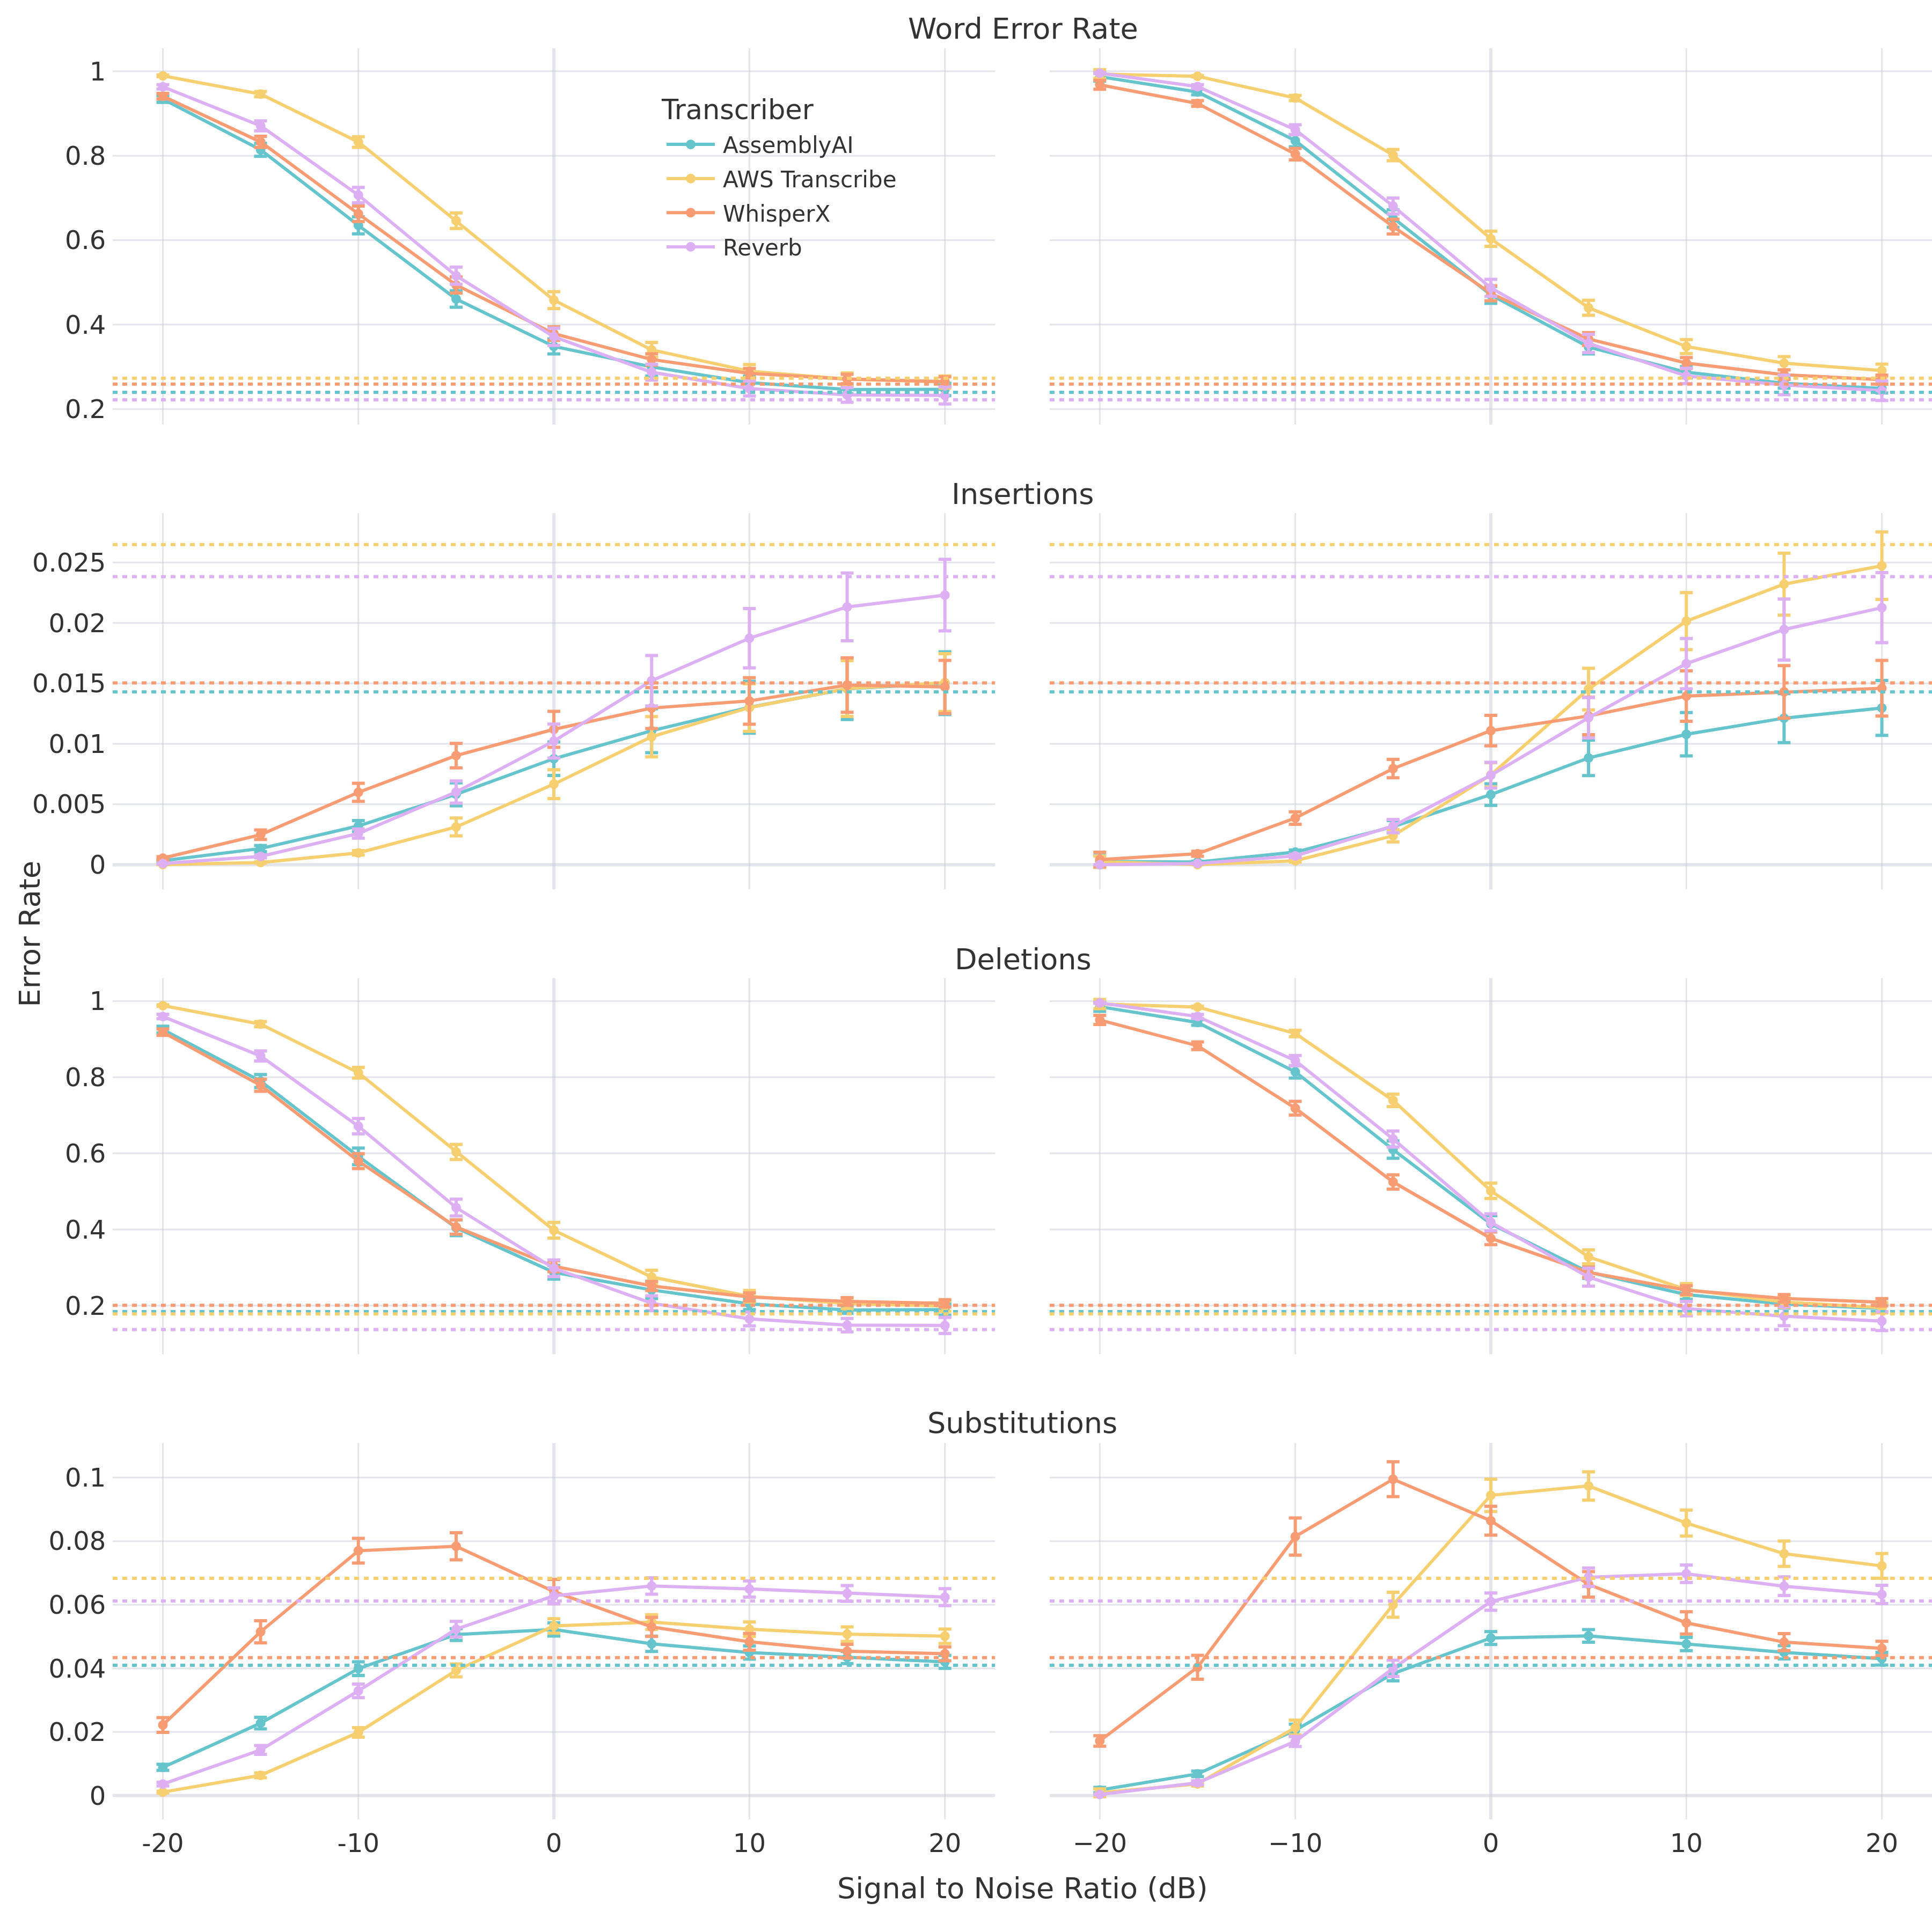
\includegraphics[width=0.98\textwidth]{figures/error_types.png}
    \caption{Effect of SNR on the types of word errors for office background noise (left) and instrumental background music (right). Error bars indicate the 95\% confidence interval. Dashed lines indicate the baseline error rate for the original audio with no added noise.}
    \label{fig:snr_errors}
%\end{wrapfigure}
\end{figure*}

The effect of SNR on word error rates for each of the two noise types and four ASR models is shown in Figure \ref{fig:snr_errors}. As expected, overall WER (top panel) tended to increase with lower SNR, especially when the background noise included instrumental music. However, there was one notable exception, where one transcriber (AWS Transcribe) did slightly better with modest amounts of background office noise added to the audio. See Table \ref{tab:statsinf20} for paired t-test statistics comparing the original audio files (no added noise) with the 20 dB SNR audio.

While the overall WERs for the four ASRs are comparable and all four show similar WERs for both types of background noise across the different SNR levels (\ref{fig:snr_errors}, top row), the \textit{types} of errors made by each model vary substantially across the range of SNR levels measured and show different error characteristics for the two noise types (\ref{fig:snr_errors}, bottom three rows). In particular, AWS and Reverb make more insertion and substitution errors, but fewer deletions than either Whisper or AWS. Whisper makes fewer deletions across all SNR levels, but makes significantly more substitution and insertion errors than the other three models, especially at modest to low SNR levels. And, AWS is more impacted by low levels of added background music relative to office noise than the other three ASRs.

\subsection{Alignment Accuracy} \label{sec:alignaccuracy}
\textbf{[Maybe these detailed examples should go to the appendix with a simple summary paragraph here?]}
Below we provide three examples to show that word-based alignment methods that globally minimize Levenshtein (edit) distance and ignore temporal information can be unreliable and sometimes lead to biased error metrics. We use "S", "D", "I", and "M" to denote "Substitution", "Deletion", "Insertion", and "Match" errors respectively. "REF" and "HYP" are used to denote "Reference" and "Hypothesis" transcriptions corresponding to the human ground-truth transcription and a given ASR model transcription, respectively. 

\textbf{Example 1.} In the case of equal Levenshtein distances (i.e. same number of I, S, and D) for two alignments, one is often preferred over the other if temporal information is considered. In this example the word "good", is temporally within a reasonable window to be matched with the corresponding "good" in the REF transcription, but is not considered a match because it does not change the Levenshtein distance.
\hfil

\begin{verbatim}
Levenshtein distance method:
aws: so we come to the 3rd meetings   i have good so in the last meeting
rev: so we come to  be   s     good and **** **** so in the last meeting
                     S   S        S   S    D    D   

Temporally constrained method:
hum: so we come to the 3rd meetings   i have good *** so in the last meeting
rev: so we come to  be   s ********   * **** good and so in the last meeting
                     S   S        D   D    D        I 

metada: {
    session: "IS1007c", SNR: np.inf, Noise: "noise1", at: 52.49 s
}
\end{verbatim}

\textbf{Example 2.} A second example where equal Levenshtein distances for two alignments where one is preferred over the other when temporal information is considered. In this example the word "so" has the following start times in REF: (76.39 , 82.12) and 82.08 in HYP and thus it would be more accurate to match the only "so" in HYP with the second "so" in the REF transcription. 
\begin{verbatim}
Levenshtein distance method:
hum: we will      talk   about the conceptual design so we okay will talk about so some i
aws: we will everybody concept  to        say     ok so ** **** **** **** ***** ** **** i
                     S       S   S          S      S     D    D    D    D     D  D    D  


Temporally constrained method:
hum: we will      talk   about the conceptual design so we okay will talk about so some i
aws: we will everybody concept  to        say     ok ** ** **** **** **** ***** so **** i
                     S       S   S          S      S  D  D    D    D    D     D       D 

metada: {
    session: "IS1007c", SNR: np.inf, Noise: "noise1", at: 68.57s
}
\end{verbatim}

\textbf{Example 3.} Sometimes an identified substitution or match in an alignment using Levenshtein distance would be replaced by an insertion or deletion if the temporal distance between the words is higher than a reasonable temporal distance. This situation will lead to WER estimates that are biased lower in alignments using only Levenshtein distance and no temporal information. In the following example a substitution on the word "so" that is identified by a Levenshtein distance alignment method should be replaced by an insertion and a deletion if we consider start time of the word "so" in hum transcription (i.e. 52.49s) and the word "ok" in aws transcription (i.e. 25.61s). 
\begin{verbatim}
Levenshtein distance method:
    hum:   so (52.49)       we (52.73) ...
    aws:   ok (25.61)   really (83.81) ...
                    S                S     
Temporally constrained method:
    hum:    *           so (52.49)  we (52.73)  ...
    aws:   ok (25.61)            *           *  ...
                    I            D           D 

metada: {
    session: "IS1007c", SNR: 0, Noise: "noise1", at: 52.49s
}
\end{verbatim}

As mentioned above, this situation can also happen for matches. In following example a match on the word "so" at 61.21 seconds identified by a Levenshtein distance alignment is obviously a mistake. The hum and aws start times for the word "so" are 61.21 and 110.33 seconds respectively which again exceeds our reasonable tolerance window for temporal distance matches. 

\begin{verbatim}
Levenshtein distance method:
    hum:   ... so  (61.21) ...
    aws:   ... so (110.33) ...
                         M 
Temporally constrained method:
    hum:    ... so  (61.21) ...
    aws:    ...           * ...
                          D  
metada: {
    session: "IS1007c", SNR: 0, Noise: "noise1", at: 61.21s
}
\end{verbatim}

\textbf{Example 4.} In case of very low SNR, high-frequency transcribed words (e.g. "the", "be", "to", "of") that do not have any corresponding matches within reasonable temporal window in the REF transcription are incorrectly matched with words far in time when minimizing Levenshtein distance and ignoring temporal information. This will again lead to a WER that is lower than it would be if temporal constraints were applied. 

\subsubsection{Temporally constrained alignment}

\subsection{Quantifying Hallucinations}
We define a hallucination as a sequence of three or more inserted or substituted words in the ASR transcript where the temporal gap between the words is no longer than one second. The one second gap was chosen to eliminate word sequences that are part of temporally disconnected utterances and is meant to reflect how a human reviewing an ASR-generated transcript would not consider consecutive words separated by a long temporal gap as part of the same utterance. In Figure \ref{fig:hallucinations} we quantify the mean number of detected hallucination sequences in different ASR models at different SNR levels over all sessions using the two different types of background noise.

To evaluate how easy it would be for a human reviewer to detect potential errors in an ASR-generated transcript, we used a perplexity metric \cite{perplexityjelinek1977,perplexityhuggingface} to compare the semantic coherence of detected hallucination sequences and sequences of human transcription of equal lengths. As shown in Figure \ref{fig:perplexity}, all four ASR models produce erroneous sequences that are as coherent as human transcription sequences. This is likely due to the fact that these ASR models use a language model at their core. This level of linguistic coherence makes these failure modes more difficult to detect than errors that create an incoherent phrase and suggests that more sophisticated algorithms are needed to detect hallucination sequences. Below we sketch two heuristics that might be used for building such algorithms.

\subsubsection{Heuristics for Hallucination Detection}
\textbf{Repetitions:} We found that repetition of words in an ASR's transcription can be a strong symptom of hallucination. However, this should be utilized with great care since it is entirely possible to have a ground truth with repetitions \textbf{[TODO: @mario please quantify this in the ami human transcripts.]}. In particular, among studied ASRs, Whisper seems to have higher tendency to produce repeated words in its hallucinations. Following example, which is verified by listening to the audio file, shows that Whisper is clearly hallucinating at 780.69 seconds of "IS1007c" session in -10 SNR condition.

\begin{verbatim}
hum @ 780.96 - 787.30: so this guy this is a nother company that provides big buttons 
                       at I see that that
aws @ 780.96 - 787.30: [no transcription]
aai @ 780.96 - 787.30: [no transcription]
wsp @ 780.69 - 787.05: so this guy this is a young man from Hawaii he is got a nice hat. 
                       he is got a nice hat. he is got a nice hat. he is got a nice hat. 
                       he is got a nice hat. he is got a nice hat. he is got a nice hat.
rev @ 780.96 - 787.30: [no transcription]
----------------------------------------------------------------------------------------
metadata: {
    session: "IS1007c", SNR: -10,  Noise: "noise1", @: 780.96s
}
\end{verbatim}

\textbf{Cross-ASR Agreements:} Another metric that can be utilized to detect ASR hallucinations is the degree to which different ASRs agree in time and content. Below we provide two examples that shows the agreement of different ASRs can greatly increase the accuracy of hallucination detection. 

\textbf{Example 1.} In this example all ASRs except wsp agree that no words were spoken at 73.01 seconds. This is a strong suggestion that Whisper is hallucinating during this time. We also checked and confirmed this both by comparison with the human reference transcription and by reviewing the relevant audio clip.
\begin{verbatim}
hum @  73.01: [no transcription]
aws @  73.01: [no transcription]
aai @  73.01: [no transcription]
wsp @  73.01: can you please
rev @  73.01: [no transcription]
--------------------------------------------------------------------------------
metada: {
    session: "IS1007c", SNR: 10, Noise: "noise1", at: 72.26s
}
\end{verbatim}

\textbf{Example 2.} A) The word "or" is transcribed by all ASRs except AWS which suggests that AWS mistranscribed a single word. B) Two ASRs (i.e. AAI and WSP) agree on the transcription of the word "decrease", while AWS and REV disagree, suggesting that they may have mistranscribed this word. C) All ASRs agree on the transcription of the words "yeah but" after the word "decrease". This is a strong symptom of human error in transcribing that audio clip. Note that we confirmed that this is indeed a case of human error by reviewing the audio clip.

\begin{verbatim}
hum @  1465.52: increase or  decrease           if
aws @  1465.64: increase our price     yeah but if 
aai @  1465.51: increase or  decrease  yeah but if
wsp @  1465.61: increase or  decrease  yeah but if
rev @  1465.56: increase or  depress   yeah but if
--------------------------------------------------
metadata: {
    session: "IS1007c", SNR: 0, Noise: "noise1", at: 1465.52s
}
\end{verbatim}

\begin{figure}[!htb]
    \centering
    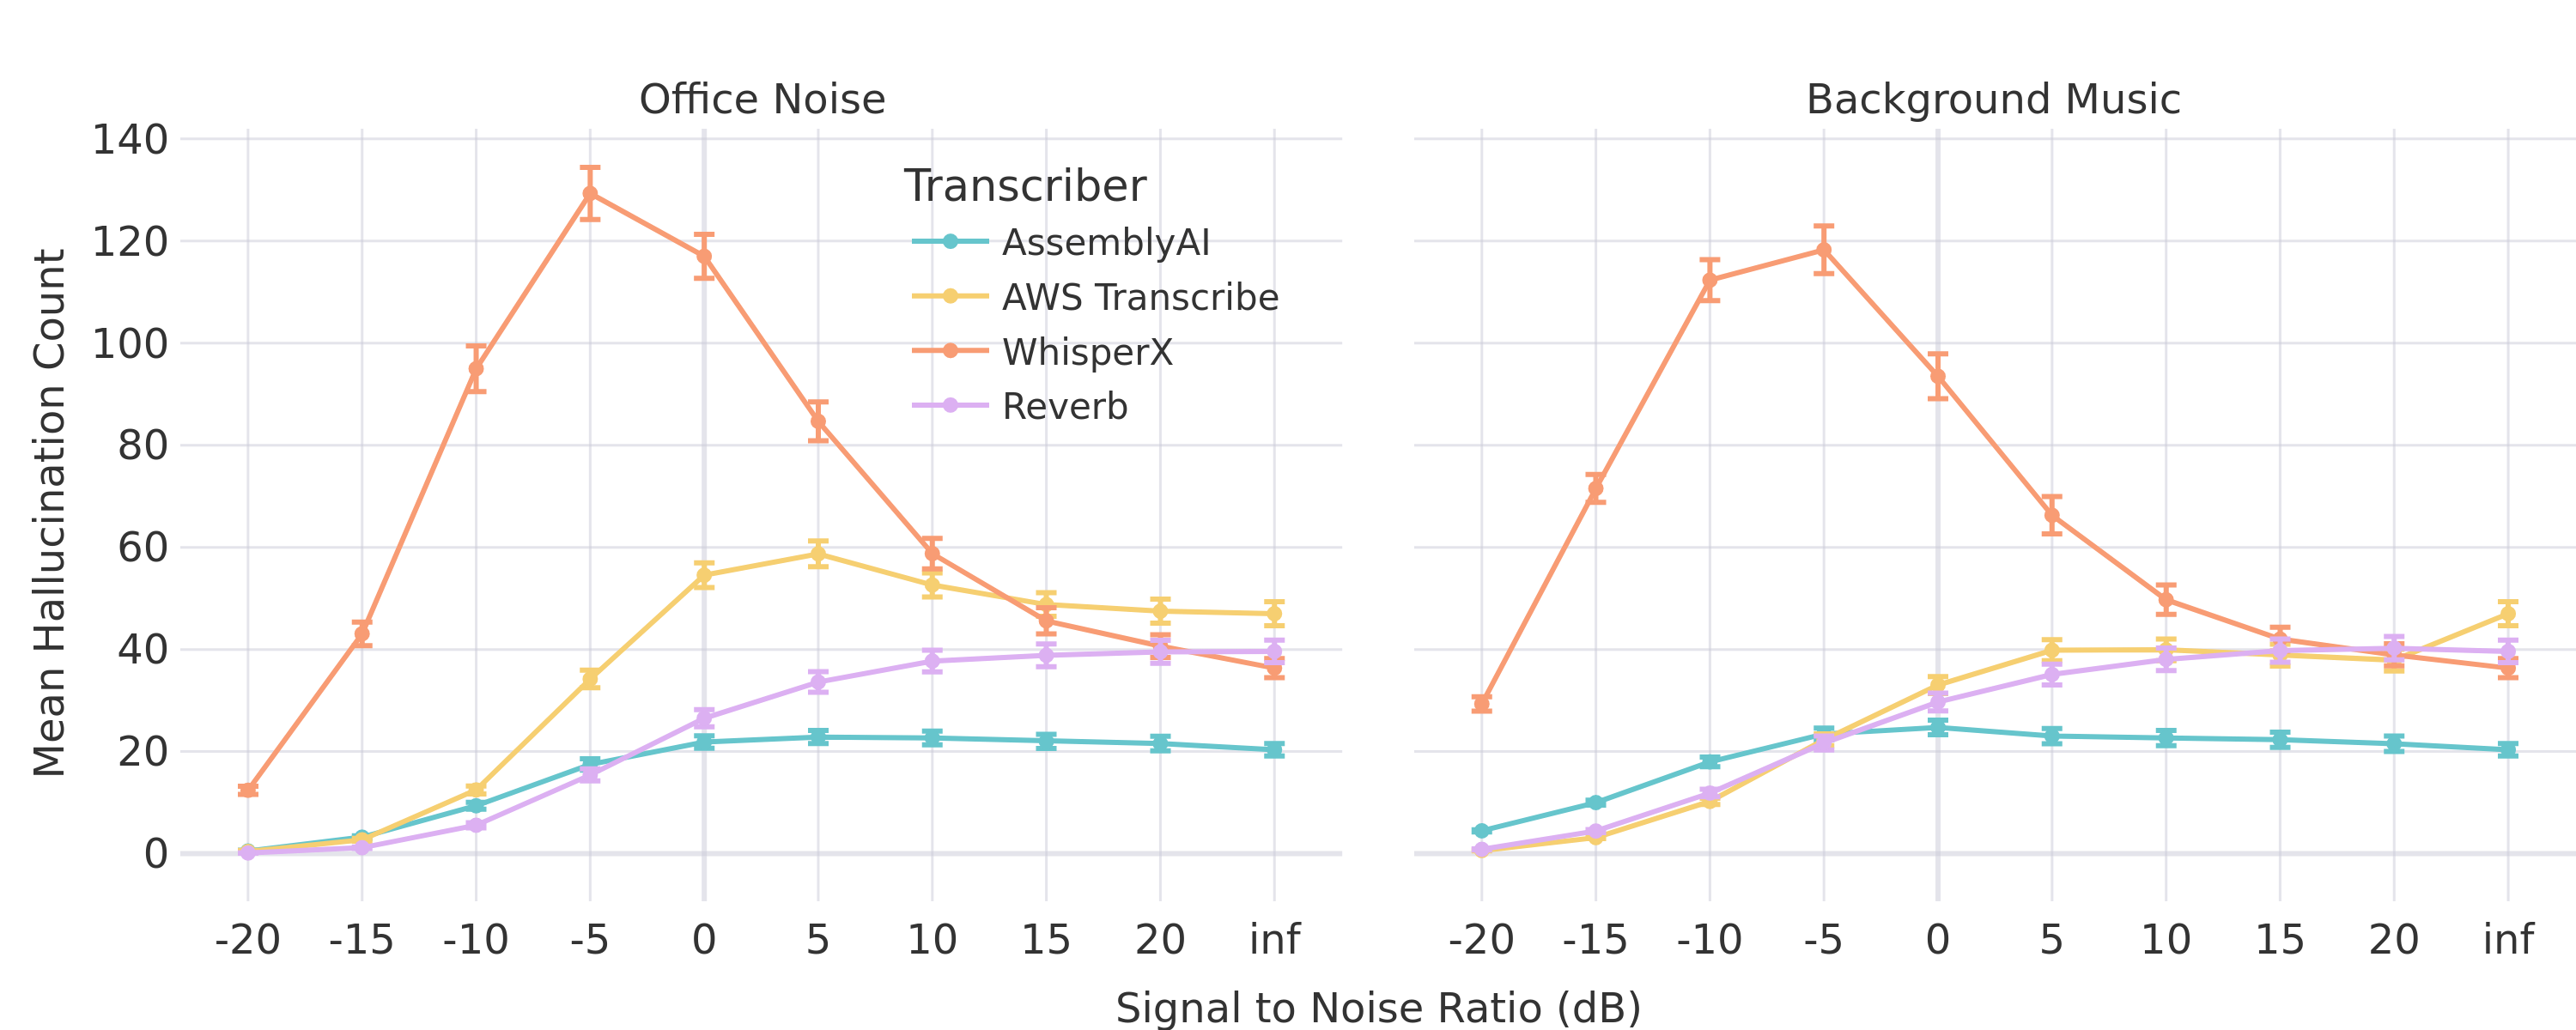
\includegraphics[width=1.0\textwidth]{figures/hallucination_count.png}
    \caption{Average number of hallucination sequences per session for the two noise types across 10 SNR levels. Error bars indicate the 95\% confidence interval. \textbf{[NOTE: plot titles are flipped-- Music is on the left.]}}
    \label{fig:hallucinations}
\end{figure}

\begin{figure}[!htb]
    \centering
    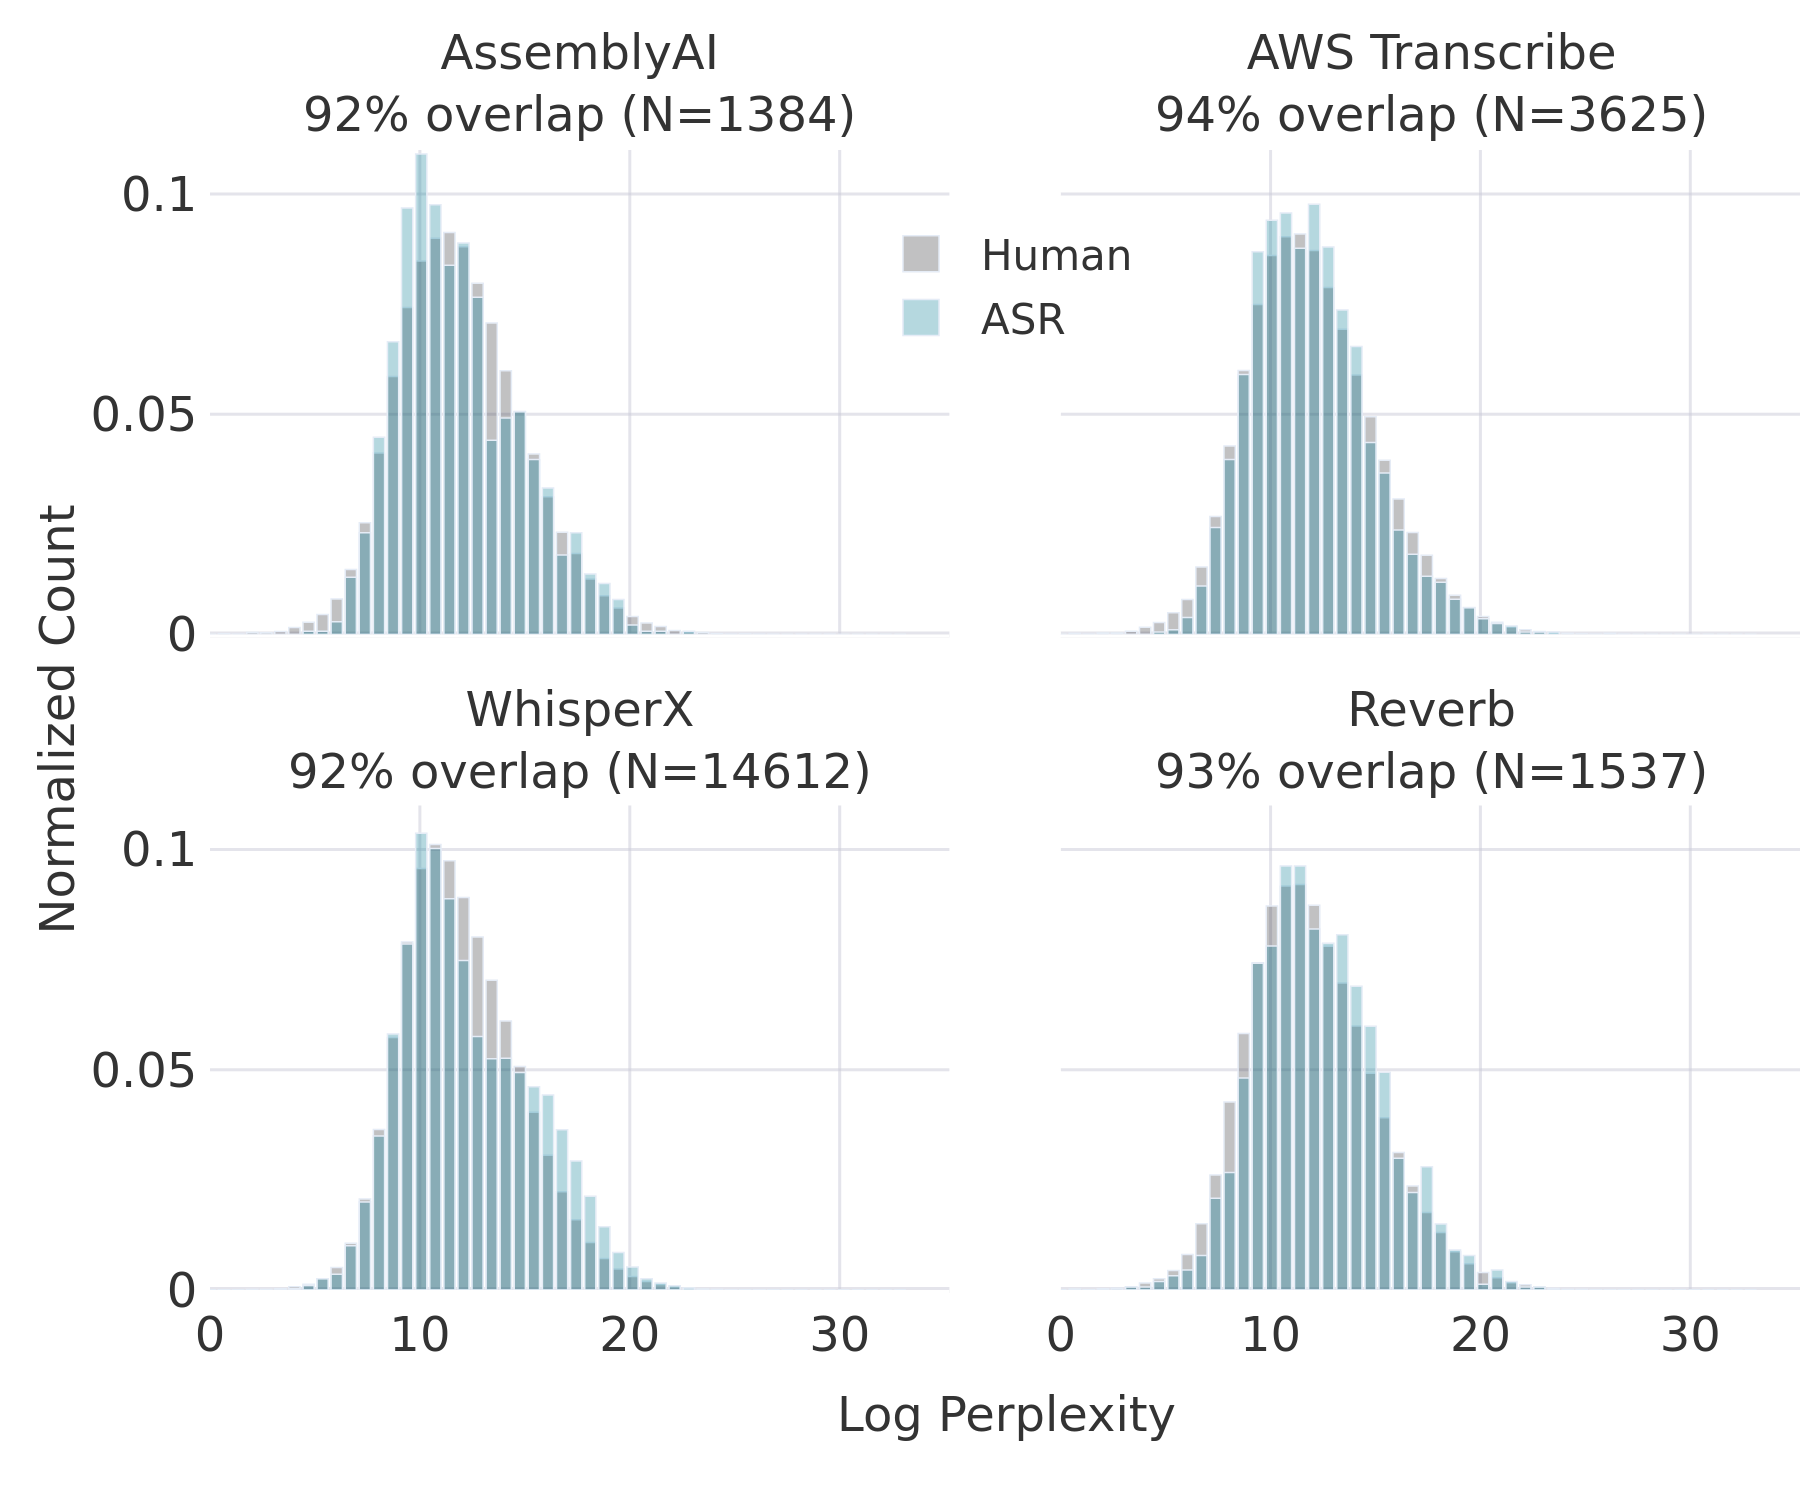
\includegraphics[width=0.7\textwidth]{figures/perplexity_distributions.png}
    \caption{Distribution of hallucination sequence log perplexities for each ASR compared to human reference perplexities for background music noise with an SNR of zero. Because perplexity is affected by the sequence length, for each sequence in a given ASR hallucination set 100 sequences of the same length were randomly selected (each without replacement) from human reference transcripts and the mean count within each bin is shown.}
    \label{fig:perplexity}
\end{figure}


\subsection{ASR word timestamp variability}
Here we evaluate the word-level timestamp accuracy of the four ASR models when no noise is added versus when moderate office noise added. As we note above, pure word-based alignments can result in temporally implausible word alignments. E.g., a common word such as "the" in an ASR transcript may align with the same word in the reference transcript that is several seconds sooner or later in time. Here we explore the extent of these temporal alignment errors.

\textbf{[BOB: I think this belongs in the appendix]}
Figure \ref{fig:jitter} shows distributions of word-level timestamp differences between the ground-truth reference transcript and the four ASR transcripts under two conditions; with no noise added (left column) and with office noise added at an SNR of zero (right column). We note that an SNR of zero is equal parts signal and noise, and in the case of office noise, the speech is audible, although not always clearly intelligible to a casual human listener. All timestamp differences are for matched words based on a standard word-based alignment that optimizes Levenschtein distance \cite{Kuhn_2023}. To evaluate the difference between normal timestamp differences between words that roughly temporally align, we plot three overlapping distributions in each panel. For the distribution labeled "all matches", timestamp differences for all matched words are considered. The ">25 matches" distribution is a subset of these timestamp differences where only matching words with more than 25 consecutive matches are considered. These words are likely to be temporally correct matches rather than spurious word alignments (e.g., common words that are temporally implausible align) and indeed the distribution of timestamp differences is much more plausible, with very few difference greater than 2 seconds. The third distribution applies the same logic, but with a more restrictive consecutive word match threshold of 50. This distribution should give a good estimate for each of the word timestamp accuracy of each of the models, as it should include very few spurious word matches. \textbf{[TODO: show a table of 99 \% quantiles for each transcriber at various consecutive word match thresholds.]}

\begin{figure}[!htb]
%\begin{wrapfigure}{R}{0.5\textwidth}
    \centering
    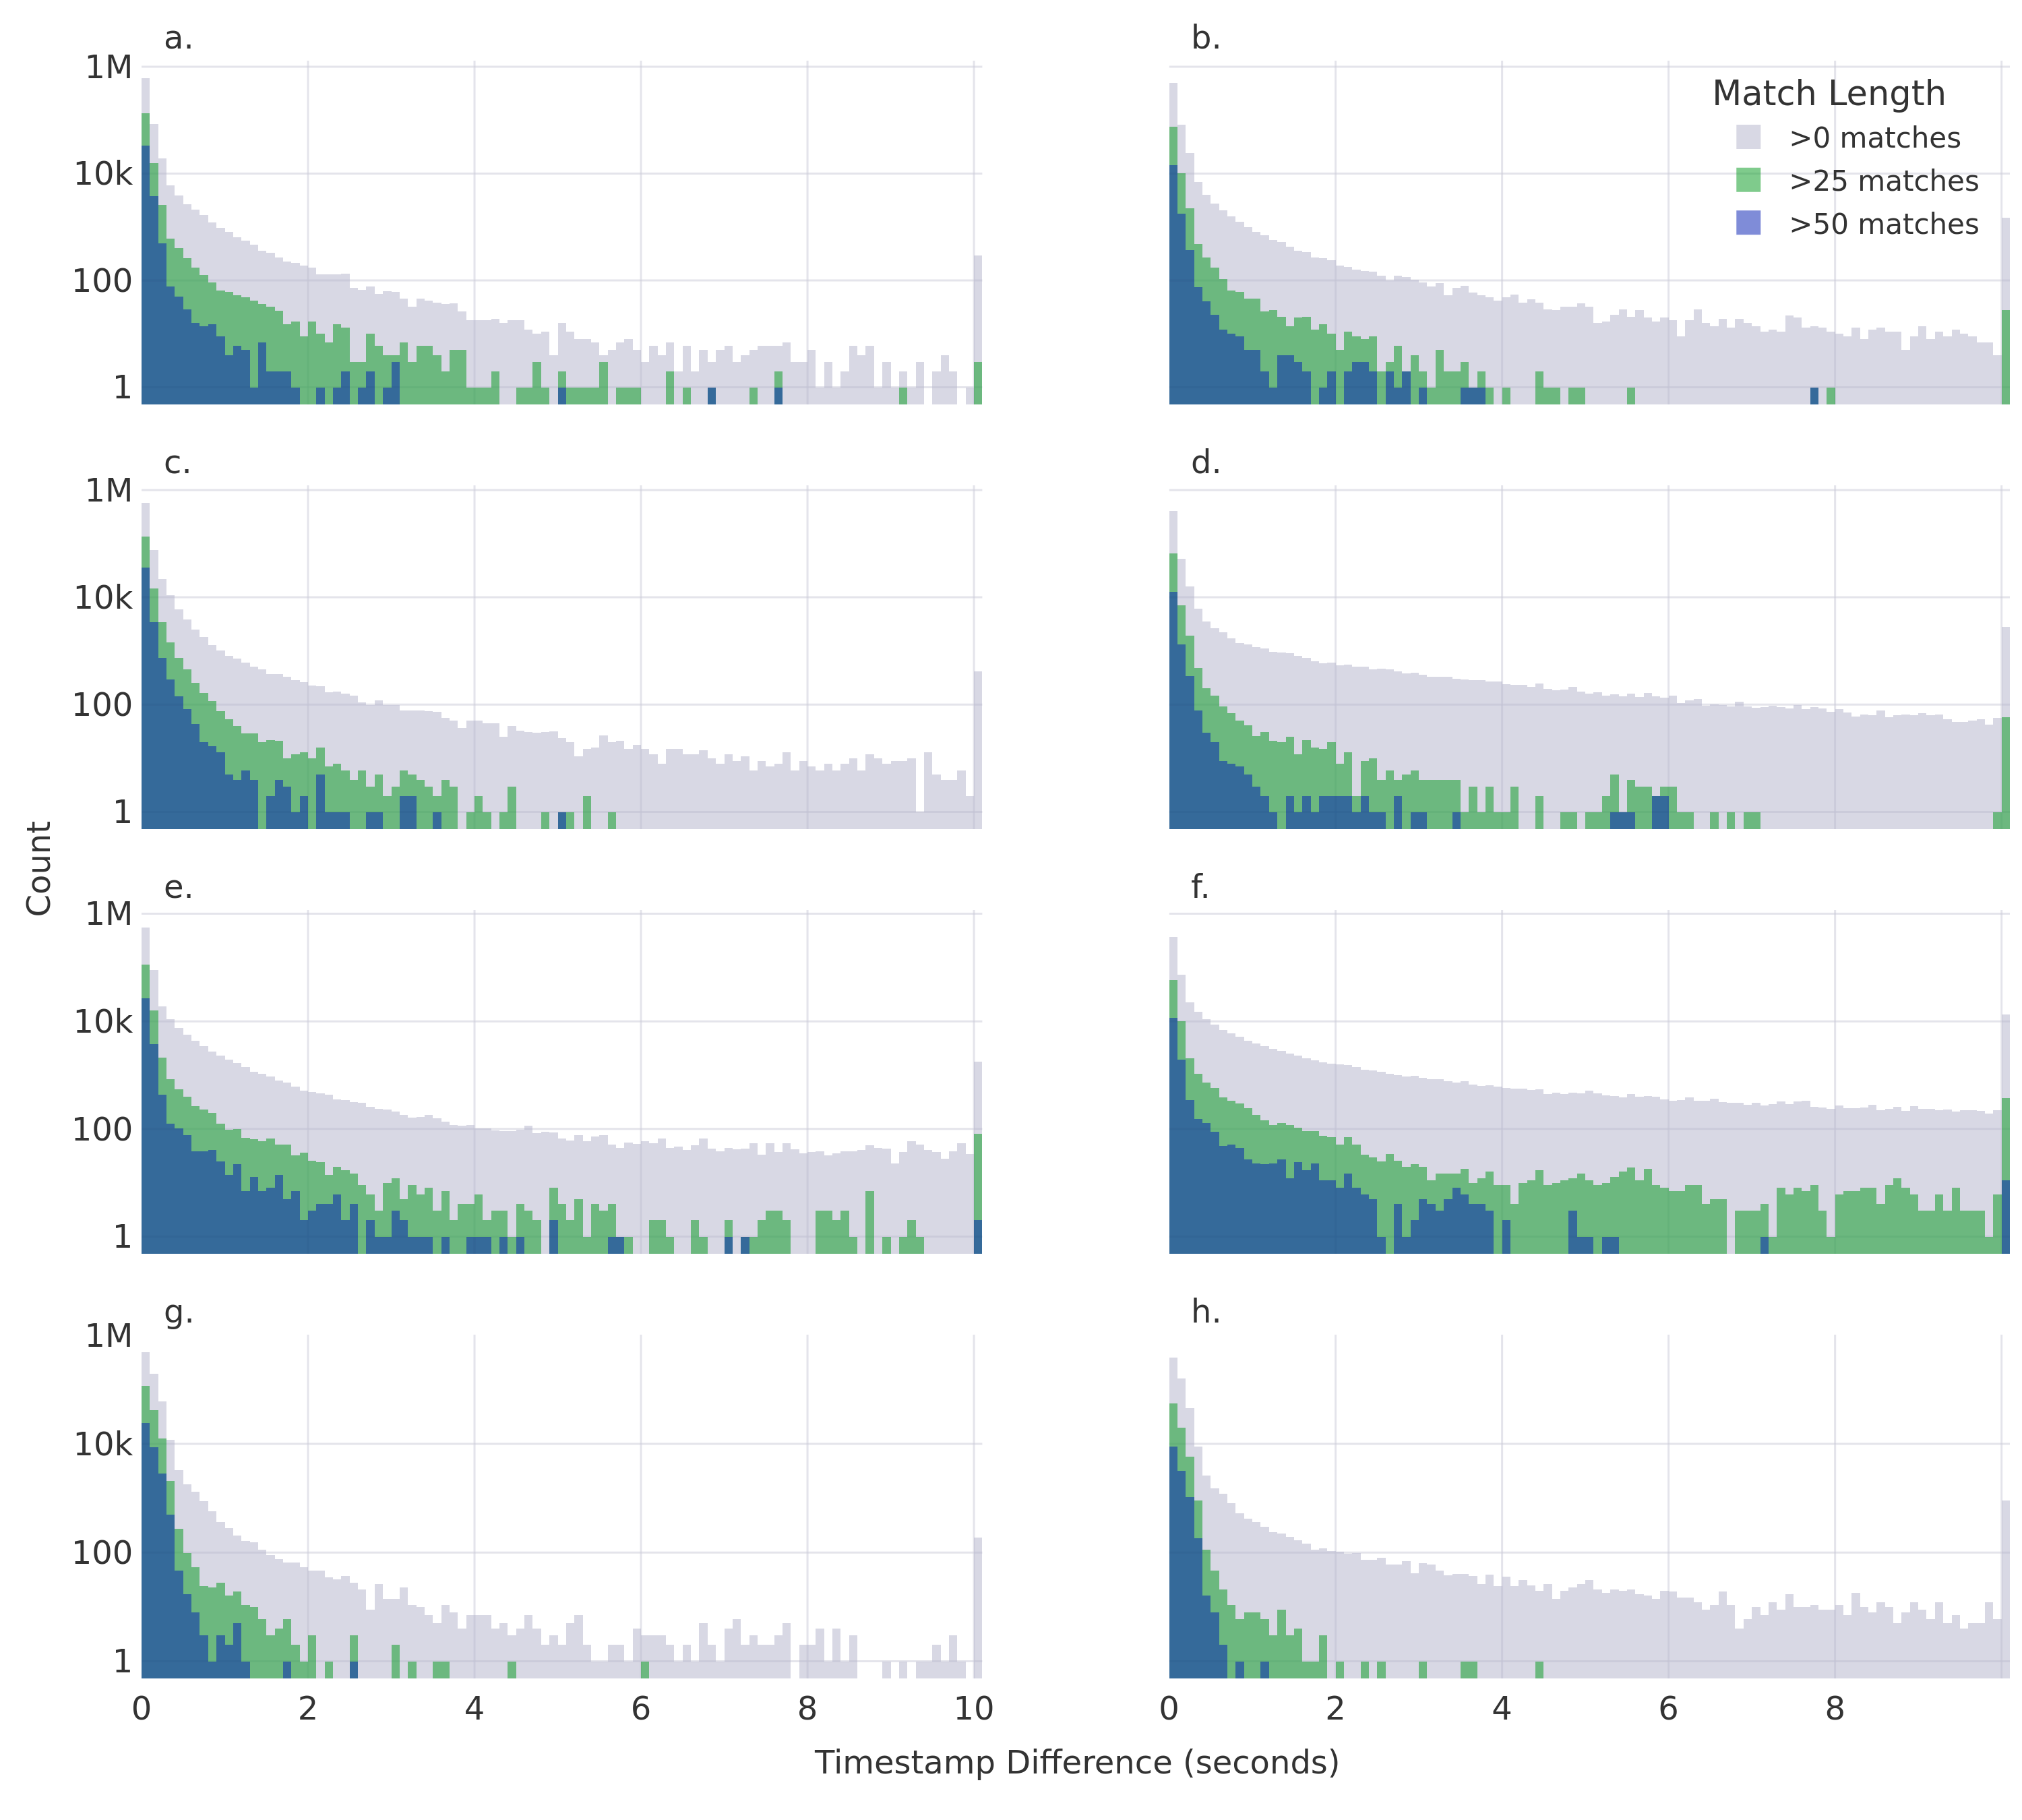
\includegraphics[width=1.0\textwidth]{figures/jitter_hist.png}
    \caption{Distributions of differences between ground-truth word timestamps and ASR timestamps using word-based alignments for three consecutive match run lengths (see legend) and for transcriptions from the original audio with no noise added (left panels; a, c, e, g) and from audio with office noise added at an SNR of 0 dB (right panel; b, d, f, h). The top row (a and b) was transcribed by AssemblyAI, the second (c and d) by AWS Transcribe, the third (e and f) by WhisperX, and the bottom (g and h) by Reverb. All data were clipped to a 10 second timestamp difference.}
    \label{fig:jitter}
%\end{wrapfigure}
\end{figure}

\section{Conclusions} 

Our systematic analysis of error patterns across multiple state-of-the-art ASR systems has implications for their application in mental health settings. By examining performance under varying levels of background noise, particularly music, we have identified distinct hallucination patterns that emerge as acoustic conditions degrade. These findings bridge a critical gap in understanding how modern generative ASR models respond to challenging audio environments commonly found in therapeutic contexts and provide an evaluation framework for ongoing evaluation of any ASR system as these models continuously improve. As we show, only looking at a top-line summary metric like WER is inadequate for properly determining which ASR system is most appropriate ASR for a given use-case because they show distinct failure modes, some of which may be more or less problematic for a given application. By systematically comparing performance across different acoustic conditions and error types, we offer a methodology that extends beyond traditional WER metrics to capture these relevant failure modes.

Future work should focus on developing ASR systems specifically optimized for mental health contexts, with robust performance in the presence of therapeutic background music. On approach worthy of exploration is using a prepossessing step that separates voice from music \cite{???}. Additionally, exploring methods to flag potential hallucinations or low-confidence segments by running multiple ASRs on the same audio file (an ASR ensemble model) could help users better interpret ASR-generated transcripts. By addressing these challenges, we can enhance the reliability of ASR-based tools in many mission-critical applications, including precision psychiatry, ultimately improving treatment fidelity evaluation, therapeutic outcome prediction, and personalized mental health care.

\textbf{[TODO: Bob to make a stronger case for why we focus on mental health applications. Psychiatry is inherently a linguistic pursuit....]}

\section{Acknowledgements}



%%%%%%%%%%%%
\bibliographystyle{unsrtnat}
\bibliography{references}

\appendix
%\renewcommand\thefigure{\thesection.\arabic{figure}}
\renewcommand\thetable{\thesection.\arabic{table}}

\clearpage
\section{Appendix 1: Data Tables}

\newcommand{\tabtext}{All t-tests (two-sided, pairwise) had 135 degrees of freedom and all p-values were adjusted for false discovery rate \cite{benjamini2001control}. Adjusted p-values less than 0.05 are shown in bold.}

\begin{table}[htp]
\centering
\label{tab:xscribersinf}
\caption{Comparing error rates across the four ASRs when no noise is added. \tabtext}
\begin{tabular}{lllllrr}
\toprule
Metric & Transcriber1 & Transcriber2 & Mean1 & Mean2 & t-statistic & p-value \\
\midrule
WER & AssemblyAI & AWS Transcribe & 0.2395 & 0.2730 & -12.10 & \textbf{ 5.4e-22} \\
  &   & WhisperX &   & 0.2590 & -14.10 & \textbf{ 5.9e-27} \\
  &   & Reverb &   & 0.2219 & 2.23 &  2.3e-01 \\
  & AWS Transcribe & WhisperX & 0.2730 & 0.2590 & 5.20 & \textbf{ 8.0e-06} \\
  &   & Reverb &   & 0.2219 & 6.05 & \textbf{ 1.6e-07} \\
  & WhisperX &   & 0.2590 &   & 4.55 & \textbf{ 1.2e-04} \\
\cmidrule(r){2-7}
Insertions & AssemblyAI & AWS Transcribe & 0.0143 & 0.0265 & -10.84 & \textbf{ 7.4e-19} \\
  &   & WhisperX &   & 0.0150 & -1.22 &  1.0e+00 \\
  &   & Reverb &   & 0.0238 & -17.33 & \textbf{ 1.2e-34} \\
  & AWS Transcribe & WhisperX & 0.0265 & 0.0150 & 9.36 & \textbf{ 3.7e-15} \\
  &   & Reverb &   & 0.0238 & 2.35 &  1.7e-01 \\
  & WhisperX &   & 0.0150 &   & -10.04 & \textbf{ 7.3e-17} \\
\cmidrule(r){2-7}
Deletions & AssemblyAI & AWS Transcribe & 0.1842 & 0.1782 & 1.90 &  4.9e-01 \\
  &   & WhisperX &   & 0.2006 & -12.63 & \textbf{ 2.5e-23} \\
  &   & Reverb &   & 0.1369 & 5.30 & \textbf{ 5.0e-06} \\
  & AWS Transcribe & WhisperX & 0.1782 & 0.2006 & -6.75 & \textbf{ 4.9e-09} \\
  &   & Reverb &   & 0.1369 & 4.42 & \textbf{ 2.0e-04} \\
  & WhisperX &   & 0.2006 &   & 6.94 & \textbf{ 1.8e-09} \\
\cmidrule(r){2-7}
Substitutions & AssemblyAI & AWS Transcribe & 0.0410 & 0.0683 & -22.63 & \textbf{ 5.7e-46} \\
  &   & WhisperX &   & 0.0434 & -5.44 & \textbf{ 2.7e-06} \\
  &   & Reverb &   & 0.0612 & -20.99 & \textbf{ 1.2e-42} \\
  & AWS Transcribe & WhisperX & 0.0683 & 0.0434 & 19.54 & \textbf{ 1.4e-39} \\
  &   & Reverb &   & 0.0612 & 5.47 & \textbf{ 2.3e-06} \\
  & WhisperX &   & 0.0434 &   & -18.06 & \textbf{ 2.6e-36} \\
\bottomrule
\end{tabular}

\end{table}

\begin{table}[htp]
\centering
\label{tab:stats_noisetype_wer}
\caption{Overall word errors for office noise vs. background music. \tabtext}
\begin{tabular}{llrrrr}
\toprule
SNR & Transcriber & Mean Office & Mean Music & t-statistic & p-value \\
\midrule
-20 & AssemblyAI & 0.93441 & 0.98729 & -7.70 & \textbf{ 3.4e-11} \\
  & AWS Transcribe & 0.98930 & 0.99356 & -0.78 &  1.0e+00 \\
  & WhisperX & 0.94109 & 0.96805 & -4.51 & \textbf{ 1.4e-04} \\
  & Reverb & 0.96330 & 0.99562 & -13.64 & \textbf{ 7.9e-26} \\
\cmidrule(r){2-6}
-15 & AssemblyAI & 0.81404 & 0.95095 & -24.59 & \textbf{ 1.0e-49} \\
  & AWS Transcribe & 0.94605 & 0.98822 & -15.83 & \textbf{ 3.9e-31} \\
  & WhisperX & 0.83273 & 0.92385 & -20.82 & \textbf{ 2.7e-42} \\
  & Reverb & 0.87078 & 0.96376 & -20.60 & \textbf{ 7.9e-42} \\
\cmidrule(r){2-6}
-10 & AssemblyAI & 0.63523 & 0.83569 & -34.95 & \textbf{ 9.3e-67} \\
  & AWS Transcribe & 0.83261 & 0.93678 & -22.95 & \textbf{ 1.4e-46} \\
  & WhisperX & 0.66246 & 0.80381 & -27.96 & \textbf{ 7.3e-56} \\
  & Reverb & 0.70680 & 0.86150 & -28.58 & \textbf{ 6.5e-57} \\
\cmidrule(r){2-6}
-5 & AssemblyAI & 0.46071 & 0.65133 & -31.54 & \textbf{ 9.5e-62} \\
  & AWS Transcribe & 0.64614 & 0.80149 & -29.84 & \textbf{ 5.0e-59} \\
  & WhisperX & 0.49390 & 0.63219 & -26.25 & \textbf{ 7.7e-53} \\
  & Reverb & 0.51576 & 0.68082 & -28.37 & \textbf{ 1.5e-56} \\
\cmidrule(r){2-6}
0 & AssemblyAI & 0.34831 & 0.47026 & -16.12 & \textbf{ 8.1e-32} \\
  & AWS Transcribe & 0.45794 & 0.60340 & -28.65 & \textbf{ 5.0e-57} \\
  & WhisperX & 0.37870 & 0.47421 & -21.38 & \textbf{ 1.9e-43} \\
  & Reverb & 0.37106 & 0.48715 & -14.51 & \textbf{ 6.0e-28} \\
\cmidrule(r){2-6}
5 & AssemblyAI & 0.29981 & 0.34681 & -4.90 & \textbf{ 2.8e-05} \\
  & AWS Transcribe & 0.34014 & 0.43986 & -23.30 & \textbf{ 2.8e-47} \\
  & WhisperX & 0.31736 & 0.36592 & -17.64 & \textbf{ 2.3e-35} \\
  & Reverb & 0.28728 & 0.35545 & -7.23 & \textbf{ 4.1e-10} \\
\cmidrule(r){2-6}
10 & AssemblyAI & 0.26253 & 0.28728 & -4.51 & \textbf{ 1.4e-04} \\
  & AWS Transcribe & 0.28965 & 0.34811 & -18.26 & \textbf{ 9.6e-37} \\
  & WhisperX & 0.28435 & 0.30888 & -13.79 & \textbf{ 3.4e-26} \\
  & Reverb & 0.24864 & 0.27836 & -3.73 & \textbf{ 2.6e-03} \\
\cmidrule(r){2-6}
15 & AssemblyAI & 0.24639 & 0.26102 & -9.13 & \textbf{ 1.3e-14} \\
  & AWS Transcribe & 0.27073 & 0.30855 & -13.12 & \textbf{ 1.5e-24} \\
  & WhisperX & 0.27108 & 0.28134 & -10.27 & \textbf{ 2.0e-17} \\
  & Reverb & 0.23343 & 0.25725 & -2.11 &  3.0e-01 \\
\cmidrule(r){2-6}
20 & AssemblyAI & 0.24657 & 0.24870 & -0.40 &  1.0e+00 \\
  & AWS Transcribe & 0.26395 & 0.29126 & -9.89 & \textbf{ 1.8e-16} \\
  & WhisperX & 0.26521 & 0.26951 & -5.94 & \textbf{ 2.6e-07} \\
  & Reverb & 0.23232 & 0.24350 & -0.86 &  1.0e+00 \\
\bottomrule
\end{tabular}

\end{table}

\begin{table}[htp]
\centering
\label{tab:stats_noisetype_ins_norm}
\caption{Insertion errors for office noise vs. background music. \tabtext}
\begin{tabular}{llrrrr}
\toprule
SNR & Transcriber & Mean Office & Mean Music & t-statistic & p-value \\
\midrule
-20 & AssemblyAI & 0.00033 & 0.00026 & 0.27 &  1.0e+00 \\
  & AWS Transcribe & 0.00001 & 0.00024 & -0.94 &  1.0e+00 \\
  & WhisperX & 0.00054 & 0.00042 & 0.37 &  1.0e+00 \\
  & Reverb & 0.00010 & 0.00000 & 5.78 & \textbf{ 5.5e-07} \\
\cmidrule(r){2-6}
-15 & AssemblyAI & 0.00133 & 0.00022 & 8.89 & \textbf{ 5.1e-14} \\
  & AWS Transcribe & 0.00018 & 0.00000 & 6.59 & \textbf{ 1.1e-08} \\
  & WhisperX & 0.00248 & 0.00090 & 10.86 & \textbf{ 6.7e-19} \\
  & Reverb & 0.00068 & 0.00010 & 10.87 & \textbf{ 6.6e-19} \\
\cmidrule(r){2-6}
-10 & AssemblyAI & 0.00320 & 0.00104 & 11.29 & \textbf{ 5.6e-20} \\
  & AWS Transcribe & 0.00098 & 0.00032 & 7.86 & \textbf{ 1.5e-11} \\
  & WhisperX & 0.00598 & 0.00386 & 7.41 & \textbf{ 1.6e-10} \\
  & Reverb & 0.00257 & 0.00072 & 11.26 & \textbf{ 6.8e-20} \\
\cmidrule(r){2-6}
-5 & AssemblyAI & 0.00582 & 0.00314 & 7.33 & \textbf{ 2.4e-10} \\
  & AWS Transcribe & 0.00312 & 0.00239 & 2.44 &  1.3e-01 \\
  & WhisperX & 0.00903 & 0.00795 & 3.10 & \textbf{ 2.1e-02} \\
  & Reverb & 0.00601 & 0.00320 & 7.37 & \textbf{ 2.0e-10} \\
\cmidrule(r){2-6}
0 & AssemblyAI & 0.00877 & 0.00580 & 5.42 & \textbf{ 2.9e-06} \\
  & AWS Transcribe & 0.00666 & 0.00743 & -1.42 &  1.0e+00 \\
  & WhisperX & 0.01120 & 0.01109 & 0.25 &  1.0e+00 \\
  & Reverb & 0.01023 & 0.00740 & 5.18 & \textbf{ 8.5e-06} \\
\cmidrule(r){2-6}
5 & AssemblyAI & 0.01108 & 0.00883 & 5.04 & \textbf{ 1.6e-05} \\
  & AWS Transcribe & 0.01059 & 0.01453 & -5.17 & \textbf{ 8.8e-06} \\
  & WhisperX & 0.01296 & 0.01231 & 1.60 &  8.9e-01 \\
  & Reverb & 0.01522 & 0.01216 & 5.15 & \textbf{ 9.8e-06} \\
\cmidrule(r){2-6}
10 & AssemblyAI & 0.01302 & 0.01079 & 4.79 & \textbf{ 4.5e-05} \\
  & AWS Transcribe & 0.01300 & 0.02015 & -8.57 & \textbf{ 3.1e-13} \\
  & WhisperX & 0.01355 & 0.01395 & -1.07 &  1.0e+00 \\
  & Reverb & 0.01874 & 0.01663 & 4.64 & \textbf{ 8.4e-05} \\
\cmidrule(r){2-6}
15 & AssemblyAI & 0.01456 & 0.01212 & 4.30 & \textbf{ 3.2e-04} \\
  & AWS Transcribe & 0.01457 & 0.02321 & -9.76 & \textbf{ 3.7e-16} \\
  & WhisperX & 0.01486 & 0.01430 & 1.28 &  1.0e+00 \\
  & Reverb & 0.02133 & 0.01946 & 4.61 & \textbf{ 9.5e-05} \\
\cmidrule(r){2-6}
20 & AssemblyAI & 0.01502 & 0.01297 & 5.44 & \textbf{ 2.7e-06} \\
  & AWS Transcribe & 0.01507 & 0.02473 & -10.74 & \textbf{ 1.4e-18} \\
  & WhisperX & 0.01471 & 0.01460 & 0.40 &  1.0e+00 \\
  & Reverb & 0.02230 & 0.02127 & 2.30 &  1.9e-01 \\
\bottomrule
\end{tabular}

\end{table}

\begin{table}[htp]
\centering
\label{tab:stats_noisetype_del_norm}
\caption{Deletion errors for office noise vs. background music. \tabtext}
\begin{tabular}{llrrrr}
\toprule
SNR & Transcriber & Mean Office & Mean Music & t-statistic & p-value \\
\midrule
-20 & AssemblyAI & 0.92520 & 0.98530 & -7.81 & \textbf{ 1.9e-11} \\
  & AWS Transcribe & 0.98821 & 0.99245 & -0.67 &  1.0e+00 \\
  & WhisperX & 0.91836 & 0.95045 & -4.77 & \textbf{ 4.8e-05} \\
  & Reverb & 0.95959 & 0.99527 & -13.59 & \textbf{ 1.0e-25} \\
\cmidrule(r){2-6}
-15 & AssemblyAI & 0.78992 & 0.94391 & -25.11 & \textbf{ 1.1e-50} \\
  & AWS Transcribe & 0.93951 & 0.98457 & -15.70 & \textbf{ 7.8e-31} \\
  & WhisperX & 0.77875 & 0.88261 & -19.86 & \textbf{ 2.8e-40} \\
  & Reverb & 0.85576 & 0.95966 & -20.80 & \textbf{ 3.0e-42} \\
\cmidrule(r){2-6}
-10 & AssemblyAI & 0.59212 & 0.81413 & -35.68 & \textbf{ 8.4e-68} \\
  & AWS Transcribe & 0.81177 & 0.91507 & -21.48 & \textbf{ 1.2e-43} \\
  & WhisperX & 0.57950 & 0.71852 & -23.40 & \textbf{ 1.9e-47} \\
  & Reverb & 0.67131 & 0.84375 & -28.76 & \textbf{ 3.3e-57} \\
\cmidrule(r){2-6}
-5 & AssemblyAI & 0.40426 & 0.60984 & -30.68 & \textbf{ 2.0e-60} \\
  & AWS Transcribe & 0.60367 & 0.73911 & -23.37 & \textbf{ 2.1e-47} \\
  & WhisperX & 0.40649 & 0.52477 & -19.62 & \textbf{ 9.6e-40} \\
  & Reverb & 0.45745 & 0.63763 & -27.74 & \textbf{ 1.7e-55} \\
\cmidrule(r){2-6}
0 & AssemblyAI & 0.28733 & 0.41492 & -15.66 & \textbf{ 9.8e-31} \\
  & AWS Transcribe & 0.39795 & 0.50157 & -17.49 & \textbf{ 5.0e-35} \\
  & WhisperX & 0.30335 & 0.37671 & -18.60 & \textbf{ 1.6e-37} \\
  & Reverb & 0.29802 & 0.41877 & -13.30 & \textbf{ 5.3e-25} \\
\cmidrule(r){2-6}
5 & AssemblyAI & 0.24102 & 0.28778 & -4.54 & \textbf{ 1.3e-04} \\
  & AWS Transcribe & 0.27501 & 0.32799 & -10.72 & \textbf{ 1.5e-18} \\
  & WhisperX & 0.25138 & 0.28721 & -15.23 & \textbf{ 1.0e-29} \\
  & Reverb & 0.20617 & 0.27463 & -6.43 & \textbf{ 2.5e-08} \\
\cmidrule(r){2-6}
10 & AssemblyAI & 0.20454 & 0.22884 & -4.10 & \textbf{ 6.7e-04} \\
  & AWS Transcribe & 0.22433 & 0.24228 & -4.64 & \textbf{ 8.4e-05} \\
  & WhisperX & 0.22247 & 0.24064 & -11.45 & \textbf{ 2.3e-20} \\
  & Reverb & 0.16495 & 0.19199 & -3.01 & \textbf{ 2.7e-02} \\
\cmidrule(r){2-6}
15 & AssemblyAI & 0.18841 & 0.20388 & -9.27 & \textbf{ 6.1e-15} \\
  & AWS Transcribe & 0.20540 & 0.20929 & -1.08 &  1.0e+00 \\
  & WhisperX & 0.21083 & 0.21879 & -8.33 & \textbf{ 1.1e-12} \\
  & Reverb & 0.14855 & 0.17198 & -1.87 &  5.2e-01 \\
\cmidrule(r){2-6}
20 & AssemblyAI & 0.18952 & 0.19270 & -0.56 &  1.0e+00 \\
  & AWS Transcribe & 0.19878 & 0.19433 & 1.27 &  1.0e+00 \\
  & WhisperX & 0.20592 & 0.20863 & -3.89 & \textbf{ 1.5e-03} \\
  & Reverb & 0.14763 & 0.15901 & -0.78 &  1.0e+00 \\
\bottomrule
\end{tabular}

\end{table}

\begin{table}[htp]
\centering
\label{tab:stats_noisetype_sub_norm}
\caption{Substitution errors for office noise vs. background music. \tabtext}
\begin{tabular}{llrrrr}
\toprule
SNR & Transcriber & Mean Office & Mean Music & t-statistic & p-value \\
\midrule
-20 & AssemblyAI & 0.00887 & 0.00173 & 11.18 & \textbf{ 1.0e-19} \\
  & AWS Transcribe & 0.00108 & 0.00088 & 0.31 &  1.0e+00 \\
  & WhisperX & 0.02219 & 0.01718 & 5.46 & \textbf{ 2.4e-06} \\
  & Reverb & 0.00361 & 0.00035 & 11.73 & \textbf{ 4.5e-21} \\
\cmidrule(r){2-6}
-15 & AssemblyAI & 0.02279 & 0.00682 & 24.10 & \textbf{ 8.6e-49} \\
  & AWS Transcribe & 0.00637 & 0.00364 & 8.29 & \textbf{ 1.4e-12} \\
  & WhisperX & 0.05150 & 0.04034 & 6.16 & \textbf{ 9.3e-08} \\
  & Reverb & 0.01433 & 0.00401 & 19.42 & \textbf{ 2.5e-39} \\
\cmidrule(r){2-6}
-10 & AssemblyAI & 0.03991 & 0.02052 & 24.97 & \textbf{ 1.9e-50} \\
  & AWS Transcribe & 0.01986 & 0.02139 & -1.74 &  6.8e-01 \\
  & WhisperX & 0.07697 & 0.08143 & -1.59 &  9.1e-01 \\
  & Reverb & 0.03292 & 0.01703 & 23.07 & \textbf{ 7.8e-47} \\
\cmidrule(r){2-6}
-5 & AssemblyAI & 0.05062 & 0.03835 & 14.09 & \textbf{ 6.3e-27} \\
  & AWS Transcribe & 0.03934 & 0.05999 & -14.56 & \textbf{ 4.5e-28} \\
  & WhisperX & 0.07839 & 0.09947 & -8.31 & \textbf{ 1.2e-12} \\
  & Reverb & 0.05231 & 0.03999 & 14.46 & \textbf{ 8.0e-28} \\
\cmidrule(r){2-6}
0 & AssemblyAI & 0.05221 & 0.04954 & 2.97 & \textbf{ 3.1e-02} \\
  & AWS Transcribe & 0.05333 & 0.09440 & -22.53 & \textbf{ 8.7e-46} \\
  & WhisperX & 0.06415 & 0.08641 & -12.83 & \textbf{ 7.9e-24} \\
  & Reverb & 0.06281 & 0.06097 & 1.70 &  7.3e-01 \\
\cmidrule(r){2-6}
5 & AssemblyAI & 0.04771 & 0.05020 & -2.75 &  5.9e-02 \\
  & AWS Transcribe & 0.05455 & 0.09734 & -27.34 & \textbf{ 8.1e-55} \\
  & WhisperX & 0.05303 & 0.06641 & -12.41 & \textbf{ 8.8e-23} \\
  & Reverb & 0.06589 & 0.06866 & -2.29 &  2.0e-01 \\
\cmidrule(r){2-6}
10 & AssemblyAI & 0.04497 & 0.04765 & -3.84 & \textbf{ 1.8e-03} \\
  & AWS Transcribe & 0.05232 & 0.08568 & -24.16 & \textbf{ 6.6e-49} \\
  & WhisperX & 0.04834 & 0.05429 & -6.99 & \textbf{ 1.4e-09} \\
  & Reverb & 0.06496 & 0.06974 & -4.67 & \textbf{ 7.3e-05} \\
\cmidrule(r){2-6}
15 & AssemblyAI & 0.04342 & 0.04502 & -3.10 & \textbf{ 2.1e-02} \\
  & AWS Transcribe & 0.05076 & 0.07605 & -19.35 & \textbf{ 3.7e-39} \\
  & WhisperX & 0.04538 & 0.04824 & -4.69 & \textbf{ 6.7e-05} \\
  & Reverb & 0.06356 & 0.06582 & -1.93 &  4.6e-01 \\
\cmidrule(r){2-6}
20 & AssemblyAI & 0.04204 & 0.04304 & -2.24 &  2.2e-01 \\
  & AWS Transcribe & 0.05010 & 0.07220 & -17.40 & \textbf{ 8.2e-35} \\
  & WhisperX & 0.04458 & 0.04629 & -5.05 & \textbf{ 1.5e-05} \\
  & Reverb & 0.06239 & 0.06323 & -0.68 &  1.0e+00 \\
\bottomrule
\end{tabular}

\end{table}

\begin{table}[htp]
\centering
\label{tab:statsinf20}
\caption{Word errors for ASR transcriptions of the original audio files (no added noise) and the 20 dB SNR audio files, including means and t-test results. All error metrics are normalized to the number of words in the human reference transcript. \tabtext}
\begin{tabular}{lllrrrr}
\toprule
Noise type & Metric & Transcriber & Mean Original & Mean SNR 20 & t-statistic & p-value \\
\midrule
Office & WER & AssemblyAI & 0.2395 & 0.2466 & -1.29 &  1.0e+00 \\
  &   & AWS Transcribe & 0.2730 & 0.2640 & 2.84 & \textbf{ 4.5e-02} \\
  &   & WhisperX & 0.2590 & 0.2652 & -3.48 & \textbf{ 6.2e-03} \\
  &   & Reverb & 0.2219 & 0.2323 & -1.12 &  1.0e+00 \\
\cmidrule(r){3-7}
  & Insertions & AssemblyAI & 0.0143 & 0.0150 & -2.56 &  1.0e-01 \\
  &   & AWS Transcribe & 0.0265 & 0.0151 & 12.08 & \textbf{ 5.7e-22} \\
  &   & WhisperX & 0.0150 & 0.0147 & 0.86 &  1.0e+00 \\
  &   & Reverb & 0.0238 & 0.0223 & 4.56 & \textbf{ 1.2e-04} \\
\cmidrule(r){3-7}
  & Deletions & AssemblyAI & 0.1842 & 0.1895 & -0.92 &  1.0e+00 \\
  &   & AWS Transcribe & 0.1782 & 0.1988 & -5.52 & \textbf{ 1.9e-06} \\
  &   & WhisperX & 0.2006 & 0.2059 & -4.15 & \textbf{ 5.6e-04} \\
  &   & Reverb & 0.1369 & 0.1476 & -1.03 &  1.0e+00 \\
\cmidrule(r){3-7}
  & Substitutions & AssemblyAI & 0.0410 & 0.0420 & -1.86 &  5.3e-01 \\
  &   & AWS Transcribe & 0.0683 & 0.0501 & 13.50 & \textbf{ 1.7e-25} \\
  &   & WhisperX & 0.0434 & 0.0446 & -1.83 &  5.6e-01 \\
  &   & Reverb & 0.0612 & 0.0624 & -1.38 &  1.0e+00 \\
\cmidrule(r){2-7}
Music & WER & AssemblyAI & 0.2395 & 0.2487 & -3.55 & \textbf{ 4.9e-03} \\
  &   & AWS Transcribe & 0.2730 & 0.2913 & -4.91 & \textbf{ 2.7e-05} \\
  &   & WhisperX & 0.2590 & 0.2695 & -6.01 & \textbf{ 1.9e-07} \\
  &   & Reverb & 0.2219 & 0.2435 & -1.92 &  4.7e-01 \\
\cmidrule(r){3-7}
  & Insertions & AssemblyAI & 0.0143 & 0.0130 & 4.45 & \textbf{ 1.8e-04} \\
  &   & AWS Transcribe & 0.0265 & 0.0247 & 6.62 & \textbf{ 9.5e-09} \\
  &   & WhisperX & 0.0150 & 0.0146 & 1.42 &  1.0e+00 \\
  &   & Reverb & 0.0238 & 0.0213 & 5.62 & \textbf{ 1.2e-06} \\
\cmidrule(r){3-7}
  & Deletions & AssemblyAI & 0.1842 & 0.1927 & -3.85 & \textbf{ 1.7e-03} \\
  &   & AWS Transcribe & 0.1782 & 0.1943 & -5.97 & \textbf{ 2.2e-07} \\
  &   & WhisperX & 0.2006 & 0.2086 & -6.64 & \textbf{ 8.4e-09} \\
  &   & Reverb & 0.1369 & 0.1590 & -1.78 &  6.3e-01 \\
\cmidrule(r){3-7}
  & Substitutions & AssemblyAI & 0.0410 & 0.0430 & -3.89 & \textbf{ 1.5e-03} \\
  &   & AWS Transcribe & 0.0683 & 0.0722 & -3.36 & \textbf{ 9.2e-03} \\
  &   & WhisperX & 0.0434 & 0.0463 & -4.24 & \textbf{ 4.0e-04} \\
  &   & Reverb & 0.0612 & 0.0632 & -2.26 &  2.1e-01 \\
\bottomrule
\end{tabular}

\end{table}

\begin{table}[htp]
\centering
\label{tab:xscribers_high_wer}
\caption{Comparing word error rates across the four ASRs for higher SNR levels. \tabtext}
\begin{tabular}{llllrr}
\toprule
Noise type & SNR & Transcriber1 & Transcriber2 & t-statistic & p-value \\
\midrule
Music & 5 & AssemblyAI & AWS Transcribe & -25.39 & \textbf{ 3.1e-51} \\
  &   &   & WhisperX & -8.34 & \textbf{ 1.1e-12} \\
  &   &   & Reverb & -1.22 &  1.0e+00 \\
  &   & AWS Transcribe & WhisperX & 18.75 & \textbf{ 7.7e-38} \\
  &   &   & Reverb & 10.61 & \textbf{ 2.8e-18} \\
  &   & WhisperX &   & 1.40 &  1.0e+00 \\
\cmidrule(r){3-6}
  & 10 & AssemblyAI & AWS Transcribe & -17.93 & \textbf{ 5.2e-36} \\
  &   &   & WhisperX & -11.17 & \textbf{ 1.1e-19} \\
  &   &   & Reverb & 1.47 &  1.0e+00 \\
  &   & AWS Transcribe & WhisperX & 10.80 & \textbf{ 9.5e-19} \\
  &   &   & Reverb & 10.02 & \textbf{ 8.3e-17} \\
  &   & WhisperX &   & 4.54 & \textbf{ 1.2e-04} \\
\cmidrule(r){3-6}
  & 15 & AssemblyAI & AWS Transcribe & -14.10 & \textbf{ 5.9e-27} \\
  &   &   & WhisperX & -11.28 & \textbf{ 5.9e-20} \\
  &   &   & Reverb & 0.38 &  1.0e+00 \\
  &   & AWS Transcribe & WhisperX & 7.54 & \textbf{ 8.2e-11} \\
  &   &   & Reverb & 5.09 & \textbf{ 1.3e-05} \\
  &   & WhisperX &   & 2.34 &  1.7e-01 \\
\cmidrule(r){3-6}
  & 20 & AssemblyAI & AWS Transcribe & -12.80 & \textbf{ 9.3e-24} \\
  &   &   & WhisperX & -12.26 & \textbf{ 2.1e-22} \\
  &   &   & Reverb & 0.51 &  1.0e+00 \\
  &   & AWS Transcribe & WhisperX & 5.75 & \textbf{ 6.4e-07} \\
  &   &   & Reverb & 4.57 & \textbf{ 1.1e-04} \\
  &   & WhisperX &   & 2.41 &  1.5e-01 \\
\cmidrule(r){2-6}
Office & 5 & AssemblyAI & AWS Transcribe & -4.25 & \textbf{ 3.9e-04} \\
  &   &   & WhisperX & -1.98 &  4.1e-01 \\
  &   &   & Reverb & 1.17 &  1.0e+00 \\
  &   & AWS Transcribe & WhisperX & 6.33 & \textbf{ 4.0e-08} \\
  &   &   & Reverb & 8.33 & \textbf{ 1.1e-12} \\
  &   & WhisperX &   & 4.71 & \textbf{ 6.1e-05} \\
\cmidrule(r){3-6}
  & 10 & AssemblyAI & AWS Transcribe & -4.66 & \textbf{ 7.7e-05} \\
  &   &   & WhisperX & -4.30 & \textbf{ 3.2e-04} \\
  &   &   & Reverb & 1.74 &  6.8e-01 \\
  &   & AWS Transcribe & WhisperX & 1.73 &  7.0e-01 \\
  &   &   & Reverb & 6.41 & \textbf{ 2.8e-08} \\
  &   & WhisperX &   & 5.45 & \textbf{ 2.6e-06} \\
\cmidrule(r){3-6}
  & 15 & AssemblyAI & AWS Transcribe & -7.33 & \textbf{ 2.4e-10} \\
  &   &   & WhisperX & -16.62 & \textbf{ 5.1e-33} \\
  &   &   & Reverb & 1.88 &  5.0e-01 \\
  &   & AWS Transcribe & WhisperX & -0.12 &  1.0e+00 \\
  &   &   & Reverb & 5.30 & \textbf{ 5.0e-06} \\
  &   & WhisperX &   & 5.29 & \textbf{ 5.3e-06} \\
\cmidrule(r){3-6}
  & 20 & AssemblyAI & AWS Transcribe & -2.87 & \textbf{ 4.1e-02} \\
  &   &   & WhisperX & -3.54 & \textbf{ 5.0e-03} \\
  &   &   & Reverb & 1.38 &  1.0e+00 \\
  &   & AWS Transcribe & WhisperX & -0.41 &  1.0e+00 \\
  &   &   & Reverb & 3.42 & \textbf{ 7.6e-03} \\
  &   & WhisperX &   & 3.64 & \textbf{ 3.6e-03} \\
\bottomrule
\end{tabular}

\end{table}

\begin{table}[htp]
\centering
\label{tab:xscribers_low_wer}
\caption{Comparing word error rates across the four ASRs for lower SNR levels. \tabtext}
\begin{tabular}{llllrr}
\toprule
Noise type & SNR & Transcriber1 & Transcriber2 & t-statistic & p-value \\
\midrule
Music & -15 & AssemblyAI & AWS Transcribe & -13.90 & \textbf{ 1.8e-26} \\
  &   &   & WhisperX & 16.58 & \textbf{ 6.2e-33} \\
  &   &   & Reverb & -9.27 & \textbf{ 6.1e-15} \\
  &   & AWS Transcribe & WhisperX & 23.11 & \textbf{ 6.5e-47} \\
  &   &   & Reverb & 14.40 & \textbf{ 1.1e-27} \\
  &   & WhisperX &   & -23.74 & \textbf{ 4.1e-48} \\
\cmidrule(r){3-6}
  & -10 & AssemblyAI & AWS Transcribe & -20.48 & \textbf{ 1.4e-41} \\
  &   &   & WhisperX & 13.65 & \textbf{ 7.3e-26} \\
  &   &   & Reverb & -12.14 & \textbf{ 4.2e-22} \\
  &   & AWS Transcribe & WhisperX & 29.64 & \textbf{ 1.1e-58} \\
  &   &   & Reverb & 20.79 & \textbf{ 3.1e-42} \\
  &   & WhisperX &   & -22.79 & \textbf{ 2.8e-46} \\
\cmidrule(r){3-6}
  & -5 & AssemblyAI & AWS Transcribe & -27.32 & \textbf{ 8.7e-55} \\
  &   &   & WhisperX & 6.30 & \textbf{ 4.7e-08} \\
  &   &   & Reverb & -12.55 & \textbf{ 3.9e-23} \\
  &   & AWS Transcribe & WhisperX & 42.19 & \textbf{ 1.9e-76} \\
  &   &   & Reverb & 26.85 & \textbf{ 6.2e-54} \\
  &   & WhisperX &   & -18.22 & \textbf{ 1.2e-36} \\
\cmidrule(r){3-6}
  & 0 & AssemblyAI & AWS Transcribe & -34.37 & \textbf{ 4.3e-66} \\
  &   &   & WhisperX & -1.65 &  8.2e-01 \\
  &   &   & Reverb & -7.81 & \textbf{ 1.9e-11} \\
  &   & AWS Transcribe & WhisperX & 34.55 & \textbf{ 2.6e-66} \\
  &   &   & Reverb & 32.03 & \textbf{ 1.7e-62} \\
  &   & WhisperX &   & -4.24 & \textbf{ 4.0e-04} \\
\cmidrule(r){2-6}
Office & -15 & AssemblyAI & AWS Transcribe & -23.80 & \textbf{ 3.1e-48} \\
  &   &   & WhisperX & -8.54 & \textbf{ 3.6e-13} \\
  &   &   & Reverb & -21.74 & \textbf{ 3.6e-44} \\
  &   & AWS Transcribe & WhisperX & 25.63 & \textbf{ 1.1e-51} \\
  &   &   & Reverb & 20.98 & \textbf{ 1.3e-42} \\
  &   & WhisperX &   & -16.86 & \textbf{ 1.4e-33} \\
\cmidrule(r){3-6}
  & -10 & AssemblyAI & AWS Transcribe & -34.30 & \textbf{ 5.2e-66} \\
  &   &   & WhisperX & -11.36 & \textbf{ 3.8e-20} \\
  &   &   & Reverb & -31.92 & \textbf{ 2.4e-62} \\
  &   & AWS Transcribe & WhisperX & 35.81 & \textbf{ 6.3e-68} \\
  &   &   & Reverb & 27.67 & \textbf{ 2.3e-55} \\
  &   & WhisperX &   & -17.56 & \textbf{ 3.5e-35} \\
\cmidrule(r){3-6}
  & -5 & AssemblyAI & AWS Transcribe & -44.33 & \textbf{ 1.1e-78} \\
  &   &   & WhisperX & -14.98 & \textbf{ 4.2e-29} \\
  &   &   & Reverb & -28.32 & \textbf{ 1.8e-56} \\
  &   & AWS Transcribe & WhisperX & 34.54 & \textbf{ 2.6e-66} \\
  &   &   & Reverb & 32.06 & \textbf{ 1.6e-62} \\
  &   & WhisperX &   & -7.41 & \textbf{ 1.6e-10} \\
\cmidrule(r){3-6}
  & 0 & AssemblyAI & AWS Transcribe & -16.68 & \textbf{ 3.6e-33} \\
  &   &   & WhisperX & -5.66 & \textbf{ 1.0e-06} \\
  &   &   & Reverb & -2.95 & \textbf{ 3.3e-02} \\
  &   & AWS Transcribe & WhisperX & 19.64 & \textbf{ 8.6e-40} \\
  &   &   & Reverb & 12.57 & \textbf{ 3.6e-23} \\
  &   & WhisperX &   & 1.20 &  1.0e+00 \\
\bottomrule
\end{tabular}

\end{table}

\end{document}